\documentclass[12pt,a4paper]{report}

\usepackage{listings}
\usepackage{xcolor}

% =========================================================
% Encoding / Fonts (Overleaf pdfLaTeX)
% =========================================================
\usepackage[utf8]{inputenc}
\usepackage[T1]{fontenc}
\usepackage{lmodern}

% =========================================================
% Page Layout / Typography
% =========================================================
\usepackage{geometry}
\geometry{margin=1in}

\usepackage{setspace}
\onehalfspacing

\usepackage{parskip}
% \usepackage{microtype} % Disabled to speed up compilation

% =========================================================
% Graphics / Tables
% =========================================================
\usepackage{graphicx}
\usepackage{float}
\usepackage{caption}
\usepackage{subcaption}

\usepackage{booktabs}
\usepackage{longtable}
\usepackage{tabularx}
\usepackage{array}
\usepackage{placeins}
% =========================================================
% Lists / Math
% =========================================================
\usepackage{enumitem}
\setlist{nosep}

\usepackage{amsmath,amssymb,bm}

% Number figures/tables/equations by section (e.g., Figure 2.1)
% \numberwithin{equation}{section}
% \numberwithin{figure}{section}
% \numberwithin{table}{section}

% =========================================================
% Headings formatting
% =========================================================
\usepackage{titlesec}
\setcounter{secnumdepth}{3}
\setcounter{tocdepth}{3}

% Clean "tab-like" gap after numbering
\titleformat{\chapter}[display]{\bfseries\huge}{\chaptername\ \thechapter}{20pt}{\Huge}
\titleformat{\section}[hang]{\bfseries\Large}{\thesection\hspace{0.9em}}{0pt}{}
\titleformat{\subsection}[hang]{\bfseries\large}{\thesubsection\hspace{0.9em}}{0pt}{}
\titleformat{\subsubsection}[hang]{\bfseries\normalsize}{\thesubsubsection\hspace{0.9em}}{0pt}{}

% =========================================================
% Table of Contents
% =========================================================
% NOTE: We intentionally avoid \texttt{tocloft} here because it can conflict with
% \texttt{titlesec} on some TeX distributions.
\renewcommand{\contentsname}{Table of contents}

% =========================================================
% Header / Footer (logo only on top-right)
% =========================================================
\usepackage{graphicx}
\usepackage{fancyhdr}

\pagestyle{fancy}
\fancyhf{}

\setlength{\headheight}{32pt}

\newsavebox{\headerlogo}
\sbox{\headerlogo}{%
  \raisebox{-0.2\height}{
\includegraphics[height=18pt]{AI_Mobile_Perception_Professional_60p_final/figures/image1.png}}%
}

\rhead{\usebox{\headerlogo}}
\lhead{}
\cfoot{\thepage}

\renewcommand{\headrulewidth}{0.4pt}

% Apply the same header/footer on chapter opening pages (plain style).
\fancypagestyle{plain}{%
  \fancyhf{}%
  \setlength{\headheight}{26pt}%
  \rhead{\usebox{\headerlogo}}%
  \cfoot{\thepage}%
  \renewcommand{\headrulewidth}{0.4pt}%
}

% =========================================================
% Figures folder
% =========================================================
% Search both the project root and the figures/ directory so that
% images render correctly in different Overleaf/project layouts.
\graphicspath{{./}{figures/}}

% =========================================================
% URLs / Hyperlinks (black)
% =========================================================
\usepackage{xurl}
\usepackage[hidelinks]{hyperref}

\begin{document}

% Avoid duplicated PDF page anchors caused by the \texttt{titlepage} environment
% resetting the page counter.
\hypersetup{pageanchor=false}

% =========================================================
% Title Page
% =========================================================
\begin{titlepage}
\centering
\vspace*{1cm}


\includegraphics[width=3cm]{AI_Mobile_Perception_Professional_60p_final/figures/image1.png}\\[1cm]

{\Large Technische Hochschule Ingolstadt\par}
\vspace{1cm}
{\huge\bfseries AI-Based Mobile Perception System\par}
\vspace{0.5cm}
{Group Project - Winter Semester 2025 - 2026}
\vspace{0.5cm}

\vfill

{\large \textbf{Project Members}: \par}
\vspace{0.3cm}
{\large
Asfak - 00170423 \\
Fatih Kiymak - 00167971 \\
Sahil - 0017XXXX \\
Sanjay - 00166686 \\
Shwetha Rai - 00173484 \par}
\vspace{0.5cm}

{\large \textbf{Supervisor}: Mr. Karthikeyan Chandrasekaran\par}
\vspace{0.2cm}

{\large Date: 06 Feb 2026\par}

\end{titlepage}

% ---------- Front matter ----------
\clearpage
\pagenumbering{roman}
\hypersetup{pageanchor=true}

\tableofcontents
\clearpage
\addcontentsline{toc}{chapter}{List of Figures}
\listoffigures
\clearpage
\addcontentsline{toc}{chapter}{List of Tables}
\listoftables
\clearpage

% =========================================================
% List of Abbreviations
% =========================================================
\chapter*{List of Abbreviations}
\addcontentsline{toc}{chapter}{List of Abbreviations}

\begin{longtable}{@{}p{0.22\textwidth}p{0.74\textwidth}@{}}
\toprule
\textbf{Abbreviation} & \textbf{Full form / description} \\
\midrule
\endhead
AI & Artificial Intelligence \\
API & Application Programming Interface \\
ASIC & Application-Specific Integrated Circuit \\
CPU & Central Processing Unit \\
CUDA & Compute Unified Device Architecture (NVIDIA GPU framework) \\
DBSCAN & Density-Based Spatial Clustering of Applications with Noise \\
FPS & Frames Per Second \\
FOV & Field of View \\
 GARD&Geometry-Informed and Uncertainty-Aware Roadside Object detection\\
GNSS & Global Navigation Satellite System \\
GPS & Global Positioning System \\
GPU & Graphics Processing Unit \\
GUI & Graphical User Interface \\
HMI & Human--Machine Interface \\
I/O & Input/Output \\
IEEE & Institute of Electrical and Electronics Engineers \\
IMU & Inertial Measurement Unit \\
IPC & Inter-Process Communication \\
JSON & JavaScript Object Notation \\
LiDAR & Light Detection and Ranging \\
ML & Machine Learning \\
NTP & Network Time Protocol \\
OSD & On-Screen Display \\
OS & Operating System \\
PCD & Point Cloud Data \\
PCL & Point Cloud Library \\
PTP & Precision Time Protocol (IEEE 1588) \\
PyQt & Python Qt Framework \\
QoS & Quality of Service \\
RAM & Random Access Memory \\
ROI & Region of Interest \\
ROS & Robot Operating System \\
ROS~2 & Robot Operating System Version 2 \\
RQt & ROS Qt-based GUI Tool \\
RViz & ROS Visualization Tool \\
SDK & Software Development Kit \\
SLAM & Simultaneous Localization and Mapping \\
TCP/IP & Transmission Control Protocol / Internet Protocol \\
TF & Transform (Coordinate Frame Relationship in ROS) \\
THI & Technische Hochschule Ingolstadt \\
UDP & User Datagram Protocol \\
UTC & Coordinated Universal Time \\
VPI & Vision Programming Interface (NVIDIA API for GPU acceleration) \\
YAML & Yet Another Markup Language \\
YOLO & You Only Look Once (Object Detection Algorithm) \\
\bottomrule
\end{longtable}

% ---------- Main matter ----------
\clearpage
\pagenumbering{arabic}

% =========================================================
% 1 Introduction
% =========================================================
\chapter{Introduction(Asfak)}


Modern intelligent surveillance and perception systems increasingly rely on the fusion of heterogeneous sensors to achieve robust and accurate situational awareness. Single-sensor systems, such as camera-only or LiDAR-only solutions, often suffer from inherent limitations including sensitivity to lighting conditions, occlusions, limited depth perception, or reduced performance in adverse environments. To overcome these challenges, multi-sensor perception systems that integrate complementary sensing modalities have become a key research and development focus in applications such as smart surveillance, autonomous systems, and intelligent infrastructure monitoring. 

The integration of Artificial Intelligence (AI) into these systems has revolutionized the ability to interpret complex sensor data in real-time. By leveraging deep learning models, particularly convolutional neural networks (CNNs), vision-based systems can now identify and track objects with high precision even in cluttered environments. Furthermore, the use of GPU acceleration on embedded platforms like NVIDIA Jetson Orin has enabled the deployment of these sophisticated models directly on the edge, reducing latency and bandwidth requirements.

This project presents the design, implementation, and evaluation of a comprehensive \textbf{AI-based Mobile Mast Perception System}. Unlike static infrastructure solutions, this system is designed for rapid deployment and high mobility, mounted on a versatile mast platform. It utilizes a sophisticated distributed architecture built on \textbf{ROS~2} (Robot Operating System 2) and is deployed across a cluster of three \textbf{NVIDIA Jetson Orin} embedded supercomputers. The sensor suite comprises a high-fidelity \textbf{RoboSense Ruby Plus 3D LiDAR} and a newly configured array of \textbf{Axis network cameras} (including Bullet, PTZ, and Panorama models), providing a full 360-degree field of view with overlapping coverage.

The core innovation of this project lies in its ability to perform accurate, real-time \textbf{2D--3D Sensor Fusion} on the edge. While cameras provide rich semantic information (classifying objects like pedestrians, cyclists, and vehicles), they lack inherent depth. Conversely, the LiDAR provides precise geometric ranging but sparse semantic data. Our system bridges this gap through a custom-built pipeline that time-synchronizes these distinct streams with microsecond precision using PTP (Precision Time Protocol), rectifies lens distortion using GPU-accelerated VPI (Vision Programming Interface), and projects 2D deep-learning detections into 3D LiDAR space.

The processing workload is strategically distributed:
\begin{itemize}
    \item \textbf{Orin~1 (Sensor Gateway):} Handles high-bandwidth acquisition from the 128-beam LiDAR and multiple camera streams.
    \item \textbf{Orin~2 (Perception Engine):} Dedicated to heavy AI workloads, running the NVIDIA VPI undistortion pipeline and the YOLOv11 deep neural network for object detection.
    \item \textbf{Orin~3 (Fusion \& Control):} Executes the multi-object tracking algorithms, global sensor fusion, and hosts the centralized control interface.
\end{itemize}

To ensure usability in the field, we have developed a custom \textbf{"Mission Control" GUI}. This interface allows operators to manage the entire distributed cluster from a single screen, visualizing data livestreams, monitoring system health, and managing data recording with a single click.

This report details the end-to-end development of this system, from the physical network configuration of the CARISSMA static IP scheme to the fine-tuning of deep learning models for urban traffic scenarios. It demonstrates how advanced edge-computing principles can be applied to create a scalable, robust, and mobile solution for next-generation intelligent transportation systems (ITS).

% =========================================================
% 2 System Background, Related Work, and Overall Pipeline
% =========================================================
\chapter[System Background]{System Background and \\ Literature Review}

This chapter establishes the theoretical and practical foundations of the AI-based mobile mast perception system. It delineates the chosen system architecture, reviews related technologies, and details the data flow pipeline—from raw sensor acquisition to fused global tracking—implemented across the distributed ROS~2 cluster.

\section{Camera-Based Perception}
Camera sensors are ubiquitous in modern perception systems, valued for their ability to capture high-resolution semantic and textural data. Deep learning-based object detectors utilize this rich visual information to classify complex traffic participants, such as pedestrians, cyclists, and vehicles, with high reliability. However, monocular cameras have a fundamental limitation: they project the three-dimensional world onto a two-dimensional plane, resulting in a loss of depth information.

Moreover, the wide-angle lenses required for surveillance coverage introduce significant radial and tangential distortion. These non-linear geometric deformations must be rigorously corrected before any precise spatial reasoning or fusion can occur. In this project, we employ a suite of Axis network cameras. To ensure geometric fidelity, their video streams are processed through a GPU-accelerated undistortion pipeline, creating a linear "pinhole" representation suitable for accurate object detection and 3D projection.

\section{LiDAR-Based Perception}
In contrast to cameras, Light Detection and Ranging (LiDAR) sensors provide direct, metrically accurate three-dimensional measurements of the environment. By emitting laser pulses and determining distance via time-of-flight, LiDARs generate dense point clouds that are largely invariant to ambient lighting conditions. This makes them indispensable for determining the precise location and size of objects.

However, LiDAR data is inherently sparse and unstructured, lacking the dense semantic texture of camera images. A cluster of points might represent a car, a bush, or a wall; without visual validation, distinguishing these can be difficult. To overcome this, our LiDAR pipeline implements a multi-stage processing chain:
\begin{itemize}
    \item \textbf{Preprocessing:} Filtering noise and removing ground plane points.
    \item \textbf{Background Subtraction:} Isolating dynamic objects from the static environment.
    \item \textbf{Clustering:} Grouping remaining foreground points into coherent object candidates.
\end{itemize}
These object clusters serve as the geometric anchor for our sensor fusion algorithm, validating and refining the semantic detections provided by the cameras.

\section{2D to 3D Localization}
Bridging the gap between the 2D image plane \textit{(u, v)} and the 3D world \textit{(x, y, z)} is a central challenge in multi-sensor perception. This process, known as 2D-to-3D localization, enables the system to assign a physical location to the objects identified by the neural network.

This project investigates two primary methodologies for this transformation:

\subsection{Approach 1: Sensor Fusion (Projection and Association)}
This method explicitly combines the strengths of both sensors. By calibrating the rigid spatial transformation (extrinsics) between the camera and LiDAR, we can mathematically project 3D LiDAR points onto the 2D camera image.
The system identifies which 3D points fall within the bounding box of a visually detected object. The depth of the object is then computed from this subset of LiDAR points. Statistical filtering is applied to reject outliers (such as background points mistakenly included in the box), ensuring a robust depth estimate. This approach is preferred for the mobile mast as it relies on active range measurement rather than geometric assumptions.

\subsection{Approach 2: Monocular Geometry (GARD)}
Methods such as "Geometry-Informed and Uncertainty-Aware Roadside Object Detection" (GARD) \cite{GARD} offer a camera-only alternative. By assuming the ground is a flat plane and strictly modeling the camera's height and pitch angle, one can solve for an object's position using ray-casting.
While computationally efficient, this method is brittle in mobile applications. Any variation in the mast's height or tilt—common occurrences during deployment or operation on uneven terrain—violates the flatness assumption and degrades accuracy. Consequently, while theoretically interesting, purely monocular approaches were deemed insufficiently robust for this project compared to the LiDAR-fusion approach.

\section{GPU-Accelerated Vision Processing}
Processing multiple high-definition video streams in real-time places a massive load on the embedded computing hardware. To prevent the CPU from becoming a bottleneck, we leveraged the hardware acceleration capabilities of the NVIDIA Jetson Orin platform.

Specifically, we utilized the NVIDIA Vision Programming Interface (VPI) to handle lens distortion correction. VPI executes this computationally intensive remapping operation on the dedicated Video Image Compositor (VIC) and Programmable Vision Accelerator (PVA) engines, bypassing the main CPU and GPU. This strategic offloading ensures that the primary GPU resources remain available for the deep learning inference tasks, maximizing total system throughput.

\section{Deep Learning-Based Object Detection}
The semantic understanding of the scene is driven by deep learning. We employ the "You Only Look Once" (YOLO) architecture, specifically the YOLOv11 variant, as our primary object detector.

\subsection{Single-Stage Architecture}
Unlike two-stage detectors (like Faster R-CNN) that first propose regions and then classify them, YOLO is a single-stage detector. It divides the image into a grid and simultaneously predicts bounding boxes and class probabilities in a single forward pass \cite{redmon2016yolo}. This architecture offers an optimal trade-off between speed and accuracy, making it ideal for the latency-sensitive environment of a robotic perception system.

\subsection{The Role of Detection}
In our pipeline, the object detector output serves as the fundamental "measurement" for higher-level logic. It answers "what is out there?" (Classification) and "roughly where is it in the frame?" (2D Localization). These semantic measurements are then passed to the fusion node to be assigned precise 3D coordinates.

\section{Distributed Perception Using ROS 2}
The system's complexity necessitated a distributed computing architecture. We split the workload across three networked NVIDIA Jetson Orin devices, orchestrated by the Robot Operating System 2 (ROS~2).
\begin{itemize}
    \item \textbf{Middleware (DDS):} Components communicate via Data Distribution Service (DDS), which handles the transparent transport of messages (images, point clouds, tracks) across the Ethernet network.
    \item \textbf{Global Parameters:} We operate on a unified ROS Domain ID to ensure visibility.
    \item \textbf{Time Synchronization:} A combination of PTP (hardware) and Chrony (software) ensures that all three computers share a synchronized microsecond-level clock.
\end{itemize}

\section{Overall System Pipeline and Flow}
The data flow is designed as a unidirectional pipeline, transforming raw sensor inputs into actionable global tracks. The architecture separates high-bandwidth acquisition from high-compute inference.

\begin{figure}[H]
    \centering
    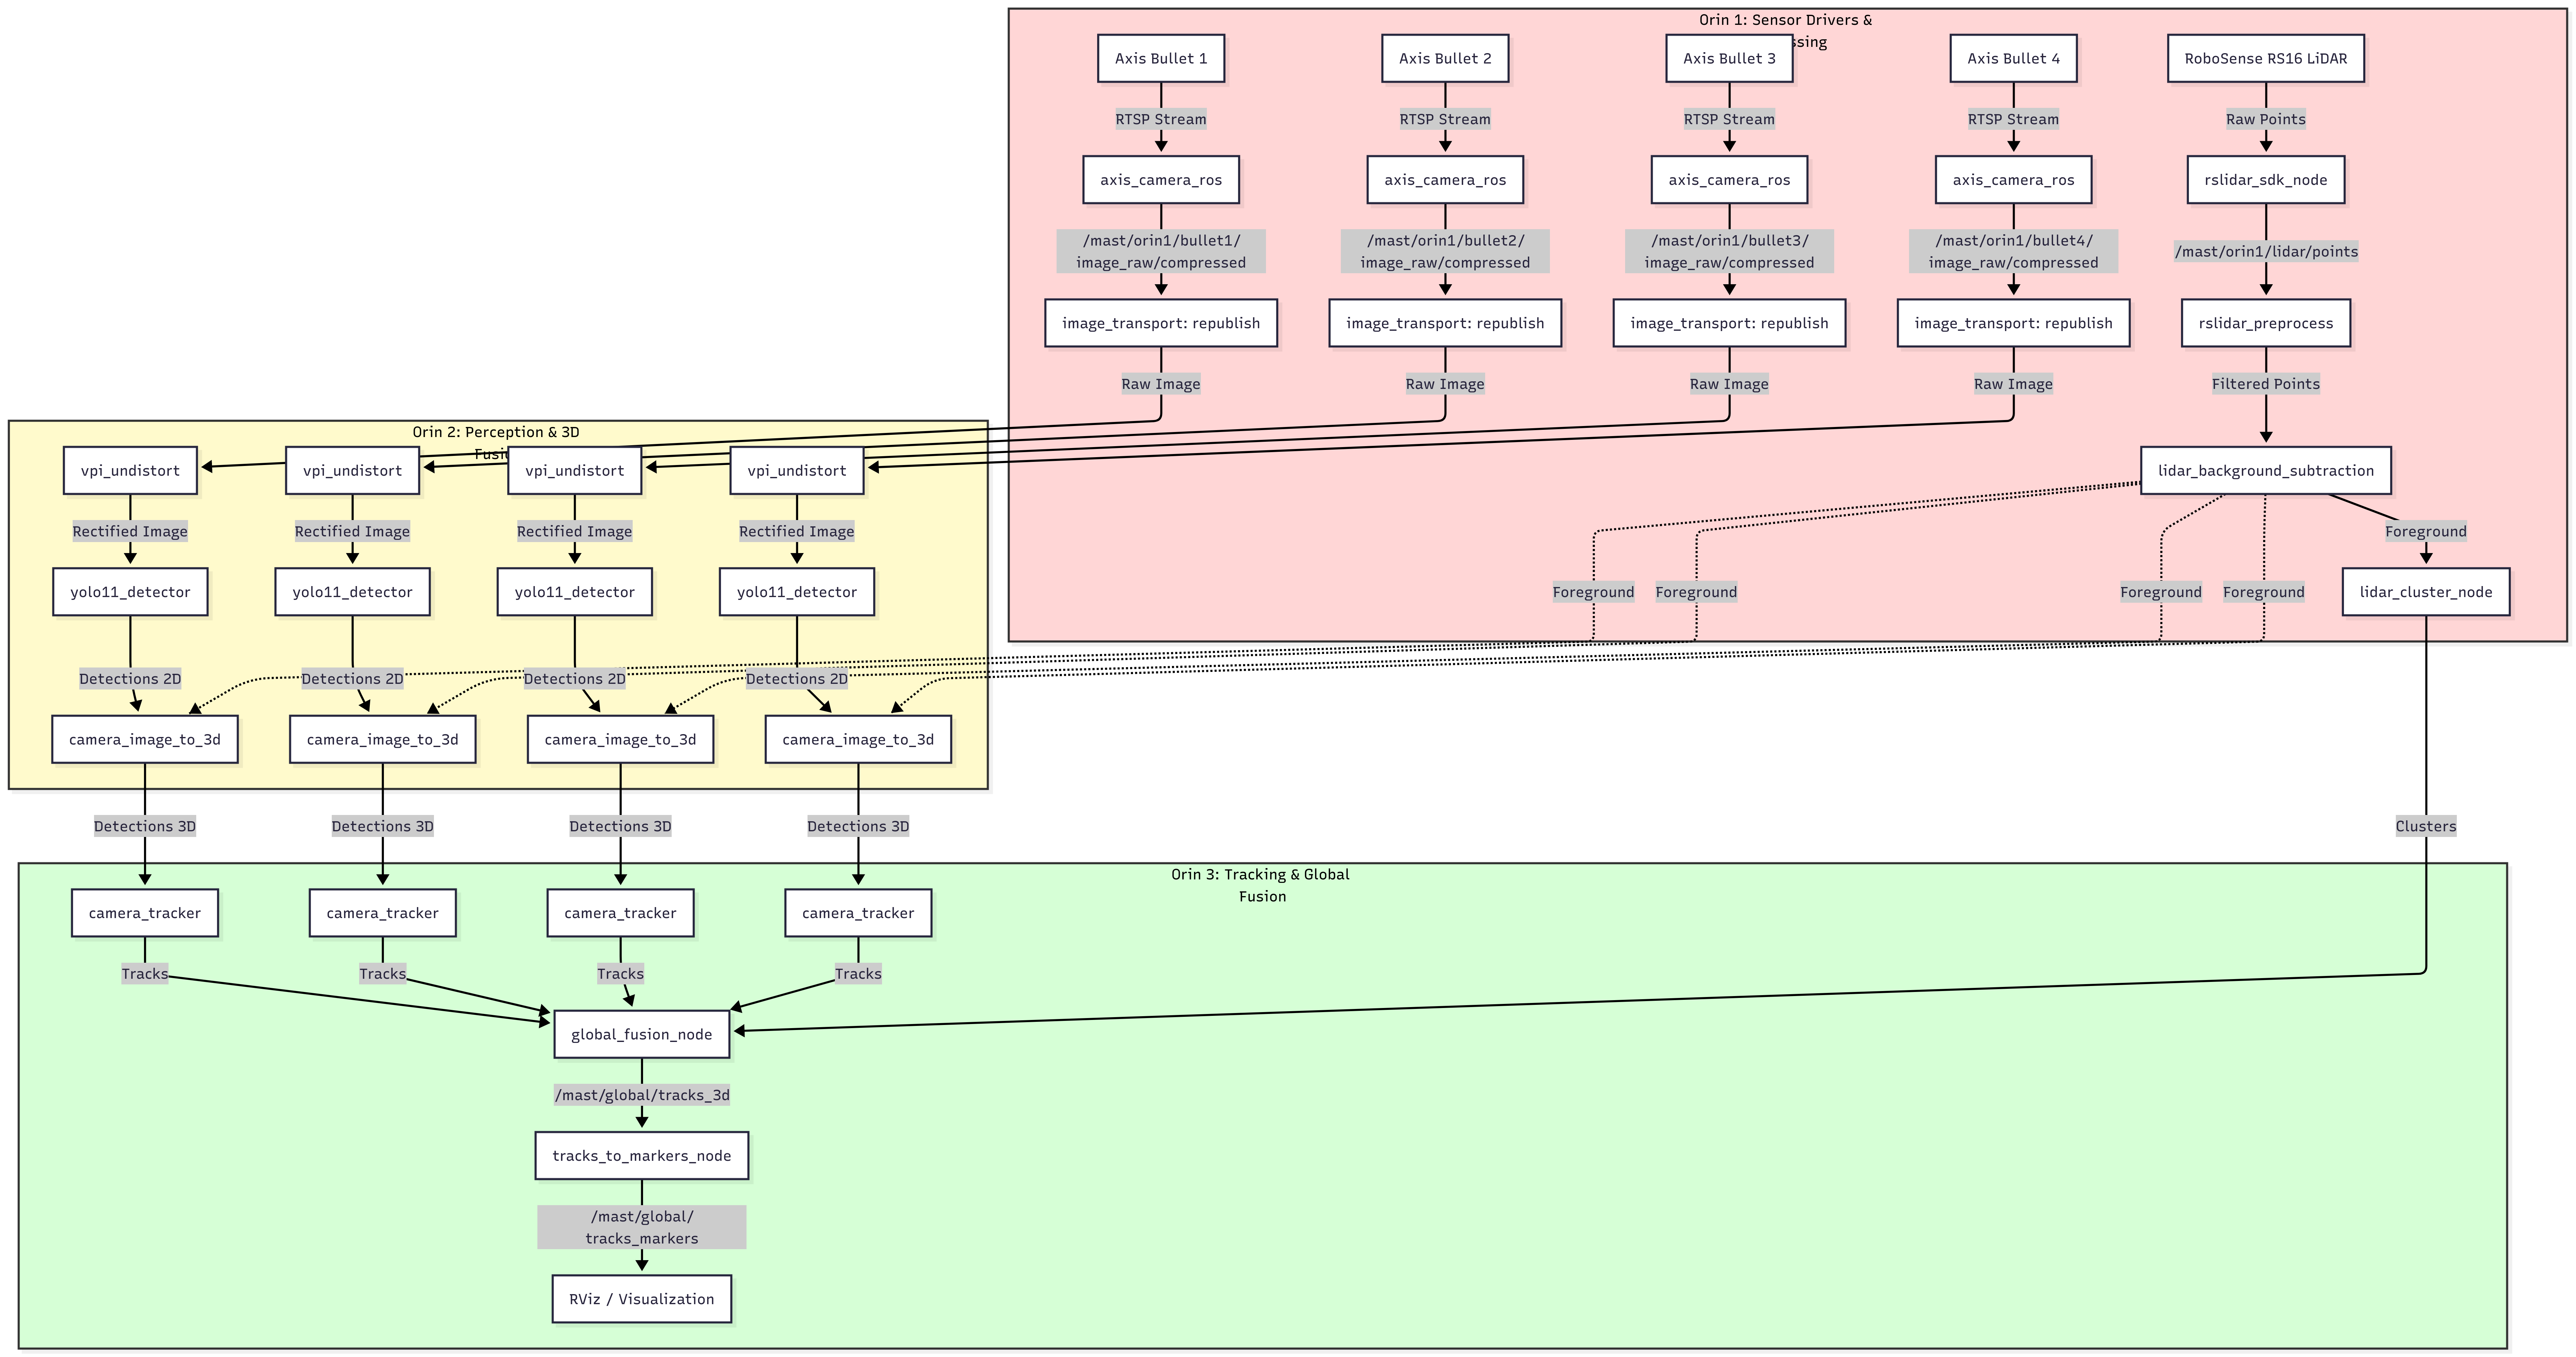
\includegraphics[width=\textwidth]{mermaid-ai-diagram-2026-01-31-205754.png}
    \caption[System Pipeline]{Complete perception pipeline across distributed Jetson Orin devices (System Diagram).}
    \label{fig:pipeline}
\end{figure}

The workload is distributed as follows:

\subsection{Orin 1: Sensor Gateway}
This device acts as the physical interface to the world. It hosts the drivers for the Axis cameras and the RoboSense LiDAR. Its primary responsibility is data ingestion and initial cleaning. It handles the high-bandwidth task of receiving network packets and publishing them as ROS topics. It also performs the first stage of LiDAR processing: filtering noise and subtracting the static background to leave only "foreground" points.

\subsection{Orin 2: Perception Engine}
The second device is the "visual cortex." It subscribes to the raw images from Orin 1. It applies the VPI undistortion to straighten the lines, and then runs the YOLO neural network to detect objects. Concurrently, it projects the LiDAR points (received from Orin 1) into these images to calculate the 3D position of each detected object. The output of Orin 2 is a stream of 3D object detections—"There is a Car at (X, Y, Z)."

\subsection{Orin 3: Fusion and Tracking}
The final device is the "associative brain." It receives the stream of instantaneous detections from Orin 2. Since detections can be noisy or intermittent, Orin 3 uses a Multi-Object Tracker (using Kalman Filters) to link these detections over time, creating smooth trajectories. It fuses redundant sightings (e.g., if two cameras see the same car) and publishes the final "Global Track List" to the user interface.

\section{ROS Parameters and Configuration}
System behavior is governed by a centralized parameter server pattern derived from ROS~2 launch files. Key configurations include:
\begin{itemize}
    \item \textbf{Network:} \texttt{ROS\_DOMAIN\_ID=0} ensures cluster-wide communication.
    \item \textbf{Camera Resoltion:} Configured to 1920x1080 at 30 FPS for optimal detail/bandwidth balance.
    \item \textbf{LiDAR:} Ports 6699 (Data) and 7788 (Info) are standard for the RoboSense driver.
    \item \textbf{TF Frames:} All spatial data is referenced to the \texttt{rslidar} frame, which serves as the origin of our mobile coordinate system.
\end{itemize}

\section{System Inputs and Outputs}
\subsection{Inputs}
\begin{itemize}
    \item \textbf{RTSP Streams:} Compressed video from Axis cameras.
    \item \textbf{UDP Packets:} Raw point data from the RoboSense LiDAR.
    \item \textbf{Calibration Data:} YAML/CSV files defining camera intrinsics and extrinsic transforms.
\end{itemize}

\subsection{Outputs}
\begin{itemize}
    \item \textbf{Global Tracks:} A list of tracked objects with IDs, positions, velocities, and classes (\texttt{/mast/global/tracks\_3d}).
    \item \textbf{Visualization:} Marker arrays for rendering in RViz.
    \item \textbf{Recordings:} Rosbag files containing the raw and processed data for offline analysis.
\end{itemize}

\section{ROS 2 Nodes and Data Flow}
The system implementation is modular, consisting of specialized nodes:
\begin{longtable}{@{}p{0.3\textwidth}p{0.65\textwidth}@{}}
\toprule
\textbf{Node} & \textbf{Function} \\
\midrule
\texttt{axis\_camera\_ros} & Captures RTSP stream and publishes compressed images. \\
\texttt{rslidar\_sdk\_node} & Driver for the LiDAR sensor; publishes point clouds. \\
\texttt{rslidar\_preprocess} & Filters point clouds (ROI, ground removal). \\
\texttt{lidar\_background\_sub} & Identifies moving objects by comparing against a static map. \\
\texttt{lidar\_cluster\_node} & Groups foreground points into distinct 3D objects. \\
\texttt{vpi\_undistort\_node} & GPU-accelerated lens correction using NVIDIA VPI. \\
\texttt{yolo\_detector\_node} & Inferencing node running YOLOv11 on TensorRT. \\
\texttt{camera\_image\_to\_3d} & Projects 2D YOLO boxes into 3D using LiDAR depth. \\
\texttt{camera\_tracker\_node} & Kalman Filter tracker for individual camera streams. \\
\texttt{global\_fusion\_node} & Aggregates tracks from all cameras into a unique global list. \\
\texttt{tracks\_to\_markers} & Visualizer node generating RViz markers. \\
\bottomrule
\end{longtable}

\section{Summary}
This chapter has outlined the architectural blueprint of the system. We have established a distributed, heterogeneous sensor processing pipeline that leverages the specific strengths of each hardware component: the semantic richness of cameras, the geometric precision of LiDAR, and the computational power of the Jetson Orin. The following chapters will detail the specific implementation of each of these subsystems.

% =========================================================
% 3 LiDAR Perception Pipeline
% =========================================================
\chapter{LiDAR Implementation}
% --- PREAMBLE SUGGESTIONS (Add these to the top of your main.tex if not present) ---
% \usepackage{listings}
% \usepackage{xcolor}
% \usepackage{hyperref}

% \lstset{


\section[LiDAR Integration]{LiDAR Hardware Integration and Drivers(Sahil)}


The implementation phase followed a rigorous two-stage integration strategy. Before deploying the software to the embedded system, I first validated the RoboSense Ruby Plus (128-beam) hardware using a standard Linux-based laptop. This ``bench test'' phase allowed me to isolate potential hardware defects and verify the driver configuration in a controlled environment before migrating the computation to the final NVIDIA Jetson Orin compute unit.

\subsection{Phase 1: Initial Hardware Verification (Linux Laptop)}
The first step involved interfacing the LiDAR hardware directly with my personal Linux workstation to verify the sensor's functionality and establish a baseline for network communication.

\textbf{Network Interface Configuration:} Since the Ruby Plus generates a massive volume of data points, establishing a stable Ethernet connection was critical. I physically connected the LiDAR’s interface box to the laptop’s Ethernet port. To enable communication, I manually configured the laptop's wired network profile to operate on the same static subnet as the sensor.

\begin{itemize}
    \item \textbf{LiDAR IP:} Verified as \texttt{192.168.6.60}.
    \item \textbf{Laptop IP:} I assigned the static address \texttt{192.168.6.50} to the laptop to act as the temporary host.
\end{itemize}

I performed a connectivity check using the \texttt{ping} command to ensure the physical link was stable.

\begin{figure}[ht!]
    \centering
    \begin{verbatim}
ping 192.168.6.60
    \end{verbatim}
    \caption{Connectivity check with LiDAR}
    \label{fig:ping_check}
\end{figure}

The response confirmed a low-latency connection ($< 1$ms), validating the physical cabling and power supply.

\textbf{Driver Setup and Visualization:} With connectivity established, I navigated to the official RoboSense website and downloaded the \texttt{rslidar\_sdk} driver package tailored for the Ruby Plus series. I created a local ROS~2 workspace on the laptop, installed the necessary build dependencies, \texttt{yaml}), and compiled the driver.

To confirm the sensor was scanning correctly, I launched the driver node and opened RViz2 on the laptop. The visualization of the point cloud confirmed that the sensor’s lasers were firing correctly and the internal motors were spinning at the desired RPM.

\subsection{Phase 2: Migration to NVIDIA Jetson Orin}
Following the successful validation on the laptop, I proceeded to migrate the software stack to the final deployment target: the NVIDIA Jetson Orin. This transition involved replicating the environment and offloading the heavy computational tasks to the Orin’s ARM-based architecture.

\textbf{Dependency Management on Orin:} I accessed the Jetson Orin via SSH and prepared the Linux environment. I manually installed the prerequisite libraries required for packet capturing, ensuring they matched the versions used during the laptop test to prevent compatibility issues:

\begin{itemize}
    
    \item \texttt{yaml file}: Essential for parsing the driver configuration files.
\end{itemize}

\textbf{Final Network Configuration:} I configured the Orin’s primary network interface to the static IP \texttt{192.168.6.1}, establishing it as the permanent gateway for the sensor suite.

% The [H] forces the image to stay right here
\begin{figure}[H]
    \centering
    \includegraphics[width=0.8\linewidth]{AI_Mobile_Perception_Professional_60p_final/figures/LiDAR Point cloud Visualization.jpeg}
    \caption{LiDAR Point Cloud Visualization Rviz2}
    \label{fig:lidar_viz}
\end{figure}

\subsection{Driver Configuration and Parameter Tuning}
The default driver configuration provided by the manufacturer is generic. To ensure optimal performance on the Orin, I explicitly tailored the \texttt{config.yaml} file located within the driver package.

\textbf{Key Configuration Changes:}
\begin{itemize}
    \item \textbf{LiDAR Type Definition:} I modified the \texttt{lidar\_type} parameter to \texttt{RS128}. This was a critical step; without this specific definition, the driver would misinterpret the data structure of the 128-beam sensor, resulting in corrupted point clouds.
    
    \item \textbf{Port Mapping:} I edited the MSOP (Data) and DIFOP (Device Info) ports to match the values \texttt{6699} and \texttt{7788}, ensuring the driver listened on the correct UDP channels mapped during the network setup.
    
    \item \textbf{Coordinate Frame:} I defined the \texttt{frame\_id} as \texttt{rslidar} to establish the root of our transformation tree.
\end{itemize}

\subsection{Node Creation and System Validation}
To finalize the integration, I created a dedicated launch file for the LiDAR node on the Orin. This node is responsible for ingesting the raw UDP packets and converting them into standard \texttt{sensor\_msgs/PointCloud2} messages for the rest of the ROS~2 system.

\textbf{Verification Steps:} Upon launching the node, I inspected the active ROS~2 topics to verify the data flow was being computed correctly by the Orin.

\begin{figure}[ht!]
    \centering
    \begin{verbatim}
ros2 topic list
ros2 topic hz /rslidar_points
    \end{verbatim}
    \caption{Verifying ROS~2 Topics and Frequency}
\end{figure}

\section{Summary}
This chapter presented the complete hardware integration and driver deployment for the LiDAR sensor. The migration of the software stack from the development laptop to the NVIDIA Jetson Orin was validated through visual confirmation in RViz, which showed the point cloud perfectly aligned with the sensor's physical environment.

While the physical integration and data streaming were successfully established, initial frequency checks revealed a significant challenge: the massive data throughput of the 128-beam sensor caused instability, preventing the system from maintaining a stable 10Hz output. The specific middleware optimizations and methodology required to resolve this bottleneck are detailed in the upcoming chapter. With the foundational hardware interface now complete, the system is prepared for the subsequent stages of the perception pipeline including preprocessing, background subtraction, and clustering to transform raw measurements into reliable object-level representations for the mobile mast application.


\section{LiDAR Time Synchronization}


Precise temporal synchronization is a fundamental requirement for multi-sensor fusion systems. In a dynamic environment, even minor timing discrepancies between the LiDAR (10 Hz) and camera (30 Hz) streams can lead to significant alignment errors (``ghosting'') when the vehicle or objects are in motion. This chapter details the engineering challenges faced in synchronizing the RoboSense Ruby Plus sensor and the transition from a hardware-based GNSS solution to a robust network-based Precision Time Protocol (PTP) architecture.

\subsection{Problem Statement: The Need for Microsecond Accuracy}
The perception system operates on a heterogeneous sensor suite. Without a unified time reference, the fusion algorithm would attempt to project 3D points onto 2D images captured at different moments in time. To mitigate this, the system requires a shared clock source (Grandmaster) that synchronizes all sensor timestamps to Universal Coordinated Time (UTC) with microsecond-level precision.

\subsection{Initial Approach: Hardware GNSS/PPS Synchronization}
Our initial design utilized a \textbf{Garmin GPS 18x LVC} receiver for hardware synchronization. This device provides two distinct signals required by the LiDAR:
\begin{enumerate}
    \item \textbf{\$GPRMC (NMEA):} A serial data stream providing the absolute UTC time.
    \item \textbf{PPS (Pulse Per Second):} A high-precision electrical pulse marking the exact start of a second.
\end{enumerate}

\subsubsection{Diagnostic Engineering: The Baud Rate Mismatch}
The GPS unit was wired to the RoboSense Interface Box, but initial tests showed an ``Unlocked'' status. To diagnose this, I developed a \textbf{temporary diagnostic node} in ROS~2 (\texttt{serial\_debugger\_node}) to analyze the raw NMEA data.
By iterating through standard baud rates (4800, 9600, 115200) within the node, I successfully decoded the NMEA sentences at 4800 bps. However, the RoboSense LiDAR firmware is hard-coded to expect NMEA data at 9600 bps. This mismatch meant the LiDAR was interpreting the valid 4800 bps GPS data as noise, preventing synchronization.

\textbf{Resolution Attempt:}
To rectify this, I interfaced the GPS with a separate utility and reprogrammed its non-volatile memory to force a 9600 bps output. While this successfully allowed the LiDAR to parse the NMEA packets, the synchronization remained intermittent due to electrical noise in the wiring harness. Consequently, this hardware-heavy approach was deemed too unreliable for the final operational environment.

\subsection[Final Solution: PTP]{Final Solution: PTP (IEEE 1588)}
To overcome the limitations of the physical GPS connection, the system was migrated to a network-based synchronization strategy using the \textbf{Precision Time Protocol (PTP)}, defined by the IEEE 1588 standard. Unlike the Network Time Protocol (NTP), which offers millisecond-level accuracy, PTP utilizes hardware timestamping at the Ethernet MAC layer to achieve sub-microsecond synchronization.

\subsubsection{Architecture Implementation}
In this architecture, the NVIDIA Jetson Orin serves as the \textbf{PTP Grandmaster Clock}, broadcasting high-precision time packets to all connected sensors over the Ethernet network.

\subsubsection{Software Configuration}
The implementation required configuring the Linux PTP stack on the compute unit and adjusting the LiDAR's internal firmware settings.

\textbf{1. Master Clock Configuration (Jetson Orin):}
I installed the \texttt{linuxptp} package and configured the \texttt{ptp4l} daemon to operate in master mode on the dedicated sensor interface (\texttt{eth0}). The configuration ensured the Orin prioritized its own system clock as the authoritative time source.

\begin{lstlisting}[language=bash, caption={Launching PTP4L in Master Mode}]
# Run PTP4L on interface eth0 in master-only mode
sudo ptp4l -i eth0 -m -4
\end{lstlisting}

\textbf{2. Slave Configuration (RoboSense LiDAR):}
Accessing the sensor's web configuration portal, I modified the \textit{Time Sync Source} parameter from ``GPS'' to ``PTP/1588''.

\subsection{Results and Validation(Sahil)}
Upon applying the PTP configuration, the synchronization stability was verified using the sensor's telemetry feedback.
\begin{itemize}
    \item \textbf{Lock Time:} The sensor achieves a ``Locked'' state within 30 seconds of boot.
    \item \textbf{Drift:} The offset between the LiDAR timestamp and the Orin system time was measured at $< 5$ microseconds.
\end{itemize}

This transition to PTP eliminated the need for external satellite visibility, allowing for reliable sensor fusion development in both indoor laboratory settings and outdoor deployment.

% =========================================================
% 4 Camera Perception and Time Synchronization Pipeline
% =========================================================
\chapter[Camera Perception Pipeline]{Camera Perception and \\ Time Synchronization Pipeline}

\section{Axis Camera System Overview(Asfak)}
Camera sensors play a critical role in perception systems by providing dense visual and semantic information about the environment. In the proposed system, Axis network cameras are used to capture continuous video streams of the surroundings from elevated viewpoints on a mobile mast. These cameras provide high-resolution imagery suitable for object detection, tracking, and multi-sensor fusion.

Unlike range sensors, cameras do not directly measure depth. Their effectiveness in multi-sensor perception systems therefore depends on accurate calibration, geometric correction, and precise temporal alignment with LiDAR measurements.

\section{Camera Data Acquisition}
\subsection{Axis Camera Hardware}
The Axis cameras used in this system are IP-based surveillance cameras equipped with wide-angle lenses. They support:
\begin{itemize}
    \item Network-based streaming
    \item Hardware timestamping
    \item High frame rate video capture
\end{itemize}
The cameras are mounted rigidly to maintain stable extrinsic relationships with the LiDAR sensor.

\subsection{RTSP Streaming}
Each Axis camera transmits video using RTSP protocols. Frames are encoded using standard video compression techniques and transmitted over Ethernet. Let $I_c(t)$ denote the camera image captured at time $t$. The camera produces a sequence:
\begin{equation}
\{ I_c(t_1), I_c(t_2), \dots, I_c(t_n) \},
\end{equation}
where $t_i$ corresponds to camera clock timestamps.

\subsection{axis\_camera\_ros Node}
\textbf{Node name:} \texttt{axis\_camera\_ros}

\textbf{Function:} Captures network video streams and publishes them as ROS~2 image messages.

\textbf{Published topics:}
\begin{itemize}
    \item \texttt{/mast/orin1/bulletX/image\_raw/compressed}
    \item \texttt{/mast/orin1/bulletX/image\_raw}
\end{itemize}

\section{Camera Image Transport and Processing}
\subsection{Compressed Image Transport}
Compressed image transport significantly reduces bandwidth usage, which is crucial for transmitting multiple high-definition streams over the network. The \texttt{axis\_camera\_ros} node publishes images in JPEG format:
\begin{itemize}
    \item \textbf{Topic:} \texttt{/mast/orin1/bulletX/image\_raw/compressed}
    \item \textbf{Format:} \texttt{jpeg}
\end{itemize}
These compressed images are efficient for monitoring but unsuitable for processing (Undistortion/YOLO) which requires raw pixel data.

\subsection{Raw Image Republishing}
To prepare images for processing, the \texttt{image\_transport} republish node decodes the compressed streams into raw \texttt{sensor\_msgs/Image} messages. This step typically runs on the processing unit (Orin 2) to keep the raw data local to the inference engine.
\begin{equation}
I_c^{\mathrm{raw}}(t) = \mathrm{Decode}\bigl(I_c^{\mathrm{comp}}(t)\bigr).
\end{equation}

\section{Camera Time Synchronization}
Accurate temporal alignment between camera images and LiDAR point clouds is essential for correct spatial association.

\subsection{LiDAR Time Reference (GPS Time)}
The LiDAR sensor operates on a GPS-disciplined clock, producing timestamps in a global time reference $T_{\mathrm{GPS}}$. LiDAR point clouds are stamped as $P_L(T_{\mathrm{GPS}})$ and used as the system master reference.

\subsection{Camera Time Alignment Strategy}
Camera timestamps $T_c$ are aligned to the LiDAR reference using an offset correction:
\begin{equation}
T_c^{\mathrm{aligned}} = T_c + \Delta T,
\end{equation}
where $\Delta T$ is the estimated clock offset between the camera and LiDAR clocks.

\subsection{Precision Time Protocol (PTP) Integration}
To minimize clock drift and offset, Precision Time Protocol (PTP) is used. The clock offset can be estimated as:
\begin{equation}
\Delta T = \frac{(t_2 - t_1) + (t_3 - t_4)}{2},
\end{equation}
where $t_1,t_2,t_3,t_4$ are PTP message timestamps.

\section{Camera Image Undistortion (NVIDIA VPI)}
Wide-angle lenses introduce non-linear distortions that affect geometric accuracy. To ensure reliable 2D--3D association, the system performs GPU-accelerated undistortion using NVIDIA VPI.

\subsection{Lens Distortion Model}
The pinhole camera model with radial and tangential distortion is used:
\begin{equation}
\begin{aligned}
x_d &= x_u (1 + k_1 r^2 + k_2 r^4 + k_3 r^6) + 2p_1 x_u y_u + p_2(r^2 + 2x_u^2), \\
y_d &= y_u (1 + k_1 r^2 + k_2 r^4 + k_3 r^6) + p_1(r^2 + 2y_u^2) + 2p_2 x_u y_u,
\end{aligned}
\end{equation}
where $r^2 = x_u^2 + y_u^2$, $(x_u,y_u)$ are undistorted normalized coordinates, and $(x_d,y_d)$ are distorted coordinates.

\subsection{GPU-Accelerated Undistortion}
VPI precomputes a \emph{WarpMap} that defines a pixel-wise mapping between rectified and distorted image coordinates. This mapping is then applied efficiently on the GPU for each frame to produce a rectified image topic:
\begin{itemize}
    \item Input: \texttt{/mast/orin1/bulletX/image\_raw}
    \item Output: \texttt{/mast/orin1/bulletX/image\_rect}
\end{itemize}

\subsection{Why NVIDIA VPI Is Used(Asfak)}
The choice of NVIDIA Vision Programming Interface (VPI) for image undistortion is driven by the need for high-throughput and low-latency processing in a multi-camera setup. Traditional CPU-based undistortion methods, such as those provided by standard OpenCV implementations, often become a bottleneck when processing multiple high-resolution streams (e.g., 1080p or 4K) at 30 FPS. 

VPI provides several critical advantages:
\begin{itemize}
    \item \textbf{Hardware Acceleration:} VPI leverages the dedicated hardware engines on the Jetson Orin, including the Programmable Vision Accelerator (PVA) and the Video Image Compositor (VIC), in addition to the GPU (via CUDA). This offloading ensures that the main GPU remains available for deep learning inference (YOLO).
    \item \textbf{Stream-Based API:} VPI's asynchronous stream-based execution model allows for overlapping memory transfers with computation, maximizing hardware utilization.
    \item \textbf{Precomputed Remap Tables:} By precomputing the WarpMap based on the camera intrinsic and distortion parameters, VPI reduces the per-frame overhead to a simple remapping operation, which is highly optimized for the Jetson hardware.
    \item \textbf{Zero-Copy Memory Access:} VPI facilitates efficient memory sharing between different hardware engines and ROS~2 image buffers, minimizing unnecessary data copies.
\end{itemize}

In our implementation, the undistortion node subscribes to the raw image topic, performs the remapping using the CUDA backend for maximum speed, and publishes the rectified image to be used by the YOLO detector. This architecture allows us to maintain a stable frame rate even with heavy computational loads.

\section{Datasets and Data Preparation(Fatih)}
In this project, multiple large-scale public datasets were combined to construct a comprehensive and diverse training set for camera-based object detection in urban traffic environments. The selected datasets cover a wide range of traffic participants, viewpoints, weather conditions, and scene complexities, which is essential for building a robust perception system suitable for real-world deployment.



\subsection{\textbf{Overview of Used Datasets} }
The project integrates several key datasets to cover a broad spectrum of traffic environments and perspectives. For infrastructure-based viewpoints, the TUMTraf A9 R1 Highway Dataset was incorporated, utilizing three distinct scenarios to capture varying traffic densities. To improve the detector’s performance under fixed-camera and mobile mast perspectives, the UA-DETRAC and VisDrone datasets were also included. In particular, VisDrone was selected to address challenging top-down viewpoints and significant object scale variations. 

The training set's diversity was further expanded by leveraging BDD100K for varied weather conditions and Cityscapes for high-quality European urban scenes. To ensure effective recognition of vulnerable road users, the EuroCity Persons dataset was utilized for its extensive pedestrian and cyclist labels. Additionally, RSUD20K was integrated for its dense object annotations, while the RGB component of the R-LiViT RGB-T Dataset was used to improve robustness under shifting illumination. By combining these heterogeneous sources, the resulting dataset provides a comprehensive foundation for complex, real-world traffic monitoring.
An overview of the datasets and their primary contributions is provided in Table~\ref{tab:datasets}.

\begin{table}[H]
\centering
\caption[Dataset Summary]{Summary of datasets used for training and evaluation}
\label{tab:datasets}
\begin{tabularx}{\textwidth}{l l >{\raggedright\arraybackslash}X}
\hline
\textbf{Dataset} & \textbf{Viewpoint / Scenario} & \textbf{Primary Contribution} \\
\hline
TUMTraf A9 Highway & Infrastructure-based, highway & Multi-scenario traffic density and long-range detection \\
UA-DETRAC & Fixed traffic cameras & Vehicle detection under surveillance-style viewpoints \\
VisDrone & Aerial / top-down & Scale variation and top-down object detection \\
BDD100K & On-board camera & Weather, illumination, and scene diversity \\
Cityscapes & Urban, European cities & High-quality annotations for urban traffic scenes \\
EuroCity Persons & Urban street-level & Pedestrian and cyclist detection (VRUs) \\
RSUD20K & Dense traffic scenes & High object density and cluttered environments \\
R-LiViT (RGB only) & Multi-condition RGB & Robustness to illumination changes \\
\hline
\end{tabularx}
\end{table}
Additionally, smaller auxiliary datasets focusing on specific object categories (e.g., motorcycles and e-scooters) were incorporated to address class imbalance issues observed in the initial training data. These datasets were treated as supplementary sources and merged carefully into the main training set.

\subsection{Dataset Integration}
Due to the heterogeneous nature of the selected datasets, a unified data integration strategy was required to prepare the data for training. Thus, all datasets were converted into a common YOLO-compatible format, a process that involved harmonizing class definitions across diverse sources and mapping dataset-specific labels to a unified class index set. In addition, unsupported or irrelevant classes were removed to ensure consistency across the combined dataset. Special care was taken to maintain a correct correspondence between images and their labels throughout the preprocessing stage, as this is essential for reliable training. After completing these preprocessing steps, all datasets were merged into a single unified dataset, referred to as \textit{global\_yolo}. This combined dataset was then used as the main training set for the object detection model.

\subsection{Annotation Formats and Conversion}
The original datasets utilized a variety of annotation formats, ranging from YOLO text and PASCAL VOC XML to various dataset-specific schemas. To standardize the training pipeline, all annotations were converted into a uniform YOLO format featuring normalized bounding box coordinates. This transformation was executed using custom conversion scripts designed to parse the original annotation files, validate bounding box integrity, and generate consistent label files across the entire integrated dataset. 

The conversion process ensured that each image had exactly one corresponding label file, invalid or empty annotations were removed and bounding boxes were correctly normalized based on image resolution.

\subsection{Training and Validation Split}
Training and validation splits were preserved according to the original dataset definitions whenever possible to avoid data leakage.  Therefore, all datasets were combined at the training level, while validation was performed on a fixed and consistent validation set. This ensured fair performance comparison across different training configurations and prevented overfitting to newly added data sources.

\subsection{Final Dataset Statistics}
Following the completion of preprocessing and integration, the final dataset comprises 201,354 images and an equivalent number of label files, representing a total of 1,293,541 annotated object instances. This unified training set contains seven distinct object classes, with the following class-to-index mapping:

\begin{itemize}
    \item 0: person
    \item 1: bicycle
    \item 2: motorcycle
    \item 3: car
    \item 4: bus
    \item 5: truck
    \item 6: e-scooter
\end{itemize}
By incorporating over 1.2 million instances, the dataset provides a high-density data foundation that allows the model to learn robust features across diverse urban environments while ensuring a large-scale representation of both dominant and minority vehicle classes.

\subsection{Dataset Configuration}
All datasets were accessed through a single unified dataset configuration file, named \texttt{global\_yolo.yaml}. This file specifies the paths to the training and validation images, as well as the unified list of object classes used during training. Using a single configuration file made it easier to manage the datasets and allowed new data to be added with minimal changes to the overall setup.

This final dataset configuration step provided a solid foundation for the deep learning–based object detection approach described in the following section.


\section{Deep Learning-Based Object Detection(Fatih)}
This section describes the deep learning–based object detection component of the camera perception pipeline. The objective is to detect relevant road users in the 2D image plane and to output class-labeled bounding boxes. These detections are subsequently consumed by downstream modules (e.g., global tracking and multi-sensor fusion) as structured semantic observations.

A YOLOv11-based single-stage detector was selected due to its favorable accuracy-latency trade-off and its practicality for real-time use on GPU-equipped systems. In the conducted experiments, the YOLOv11s model variant was employed as a compact baseline that balances detection performance with computational constraints.

\subsection{Detection Output and Interface}
For each RGB image frame, the detector produces a set of detections. Each detection contains a class label (from the predefined traffic-related categories), a confidence score indicating the model’s certainty and a 2D bounding box in pixel coordinates (top-left and bottom-right corners).

The detector therefore performs both classification (“what object is present?”) and localization (“where is it in the image?”). The output is formatted in a standard object-detection representation that enables straightforward integration into later perception stages, where detections can be associated over time and across sensors.




\subsection[Training Configuration]{Training Configuration and Practical Considerations}

The final training run was configured to improve detection quality on a diverse merged dataset (\textit{global\_yolo}), which includes multiple traffic datasets. For improved small-object detection and more robust localization, the input resolution was increased from the earlier 640 setting to imgsz = 960.

A representative training configuration is summarized below (as described in the experiment logs):

\begin{itemize}
    \item Model initialization: trained starting from a previously obtained best checkpoint (transfer learning).
    \item Input size: 960 × 960
    \item Batch size: 8
    \item Early stopping: enabled (patience = 10) to prevent unnecessary training once validation performance saturates.
    \item Caching: caching-to-RAM was attempted; however, system RAM was insufficient for full caching, and partial/no caching was applied automatically (as indicated by runtime warnings).
    \item Label integrity checks: duplicate labels were detected in parts of the dataset and automatically removed by the training pipeline. This indicates that label sanitation was handled during training, reducing annotation noise.
\end{itemize}

 
\subsection{Fine-Tuning and Class-Specific Improvements}
Initial training experiments revealed that certain minority classes (most notably motorcycles and e-scooters) exhibited lower recall compared to dominant vehicle classes such as cars and buses. This behavior is common in traffic datasets due to inherent class imbalance. To address this issue, targeted fine-tuning for both motorcycle and e-scooter instances was conducted by incorporating additional class-specific training samples and selectively freezing early network layers. Specifically, additional datasets focused on these minority categories were integrated into the training set. Subsequently, training was resumed from pre-trained weights instead of starting from scratch, and training schedules were adjusted to allow the model to adapt to the newly introduced data without degrading overall performance. These steps resulted in a measurable improvement in detection stability for motorcycles and e-scooters while preserving strong performance for other classes.

\subsection{Quantitative Results and Interpretation}
Model performance was evaluated using standard object detection metrics\cite{everingham2010pascal}:

\begin{itemize}
    \item Precision (P): fraction of predicted boxes that are correct.
    \item Recall (R): fraction of ground-truth objects that are detected.
    \item mAP@0.50: mean Average Precision at IoU threshold 0.50 (moderate localization requirement).
    \item mAP@0.50:0.95: mAP averaged over stricter IoU thresholds (more demanding localization quality).
\end{itemize}
The aggregated validation metrics for the final YOLOv11s run are presented in Table 4.7.1.

\begin{table}[H]
\centering
\caption[Validation metrics]{Validation metrics of the final YOLOv11s model trained with imgsz=960.}
\label{tab:values}
\begin{tabular}{lll}
\hline
\textbf{Metric} & \textbf{Value} \\
\hline
Precision & 0.48 \\
Recall & 0.54 \\
mAP@0.50 & 0.48 \\
mAP@0.50:0.95 & 0.36 \\
\hline
\end{tabular}
\end{table}
The validation results  indicate that the detector achieves a moderate overall accuracy, with recall being slightly higher than precision. This suggests that the model is capable of detecting a large portion of objects, while still producing a non-negligible number of false positives. The gap between mAP@0.50 and mAP@0.50:0.95 further suggests that localization quality under stricter IoU thresholds remains challenging, which is typical in large-scale multi-source datasets and small-object scenarios. 

\subsection{Precision–Recall and F1 Curve Analysis}
To further analyze the behavior of the trained model across different confidence thresholds, precision–recall (PR), F1-score, precision, and recall curves were examined. These curves provide insight into the trade-off between detection accuracy and completeness and help assess the stability of the model beyond single-point metrics.

\begin{figure}[!htbp]
  \centering
  \begin{subfigure}[t]{0.48\linewidth}
    \centering
    \includegraphics[width=\linewidth]{figures/BoxPR_curve.png}
    \caption{PR curve}
    \label{fig:boxpr}
  \end{subfigure}
  \hfill
  \begin{subfigure}[t]{0.48\linewidth}
    \centering
    \includegraphics[width=\linewidth]{figures/BoxF1_curve.png}
    \caption{F1--confidence curve}
    \label{fig:boxf1}
  \end{subfigure}
  \caption{Confidence-threshold analysis for the trained YOLO detector.}
  \label{fig:pr_f1}
\end{figure}

As shown in Figure~\ref{fig:pr_f1}, the PR curve depicts the inverse relationship between precision and recall, a characteristic behavior in complex object detection tasks. The F1 curve highlights the operating region where precision and recall are balanced, indicating a suitable confidence threshold for deployment. Thus, the observed curves suggest that the detector maintains stable performance across a reasonable range of confidence values, without abrupt degradation in either precision or recall.

Overall, this analysis supports the robustness of the trained model and justifies the selected confidence threshold used during the evaluation and deployment preparation.

\subsection{Analysis of Training Curves}
The training and validation dynamics are summarized in the results plot shown in Figure~\ref{fig:results}, which includes box loss, classification loss, and distribution focal loss, as well as precision, recall, and mAP curves over training epochs.

\begin{figure}[H]
    \centering
    \includegraphics[width=0.90\linewidth]{AI_Mobile_Perception_Professional_60p_final/figures/results.png}
    \caption{Training/validation losses and detection metrics over epochs for the final YOLOv11s run.}
    \label{fig:results}
\end{figure}


Based on the trends observed in Figure~\ref{fig:results} , training losses decrease rapidly during the early epochs and then plateau, indicating fast convergence under transfer learning. Validation mAP reaches its peak relatively early, around the epoch where the best checkpoint is saved, and does not improve significantly afterward, which explains the activation of early stopping. Additionally, the metric curves exhibit noticeable fluctuations, which is expected in heterogeneous datasets composed of multiple sources, where domain shift and class imbalance can lead to noisy validation signals. 


\subsection{Normalized Confusion Matrix}
The normalized confusion matrix shown in Figure~\ref{fig:confusionmatrix} provides insights into which object classes are most frequently confused by the model. Since the matrix is normalized, each column reflects how true instances of a given class are distributed across the predicted classes. 
\begin{figure}[H]
    \centering
    \includegraphics[width=0.90\linewidth]{AI_Mobile_Perception_Professional_60p_final/figures/confusion_matrix_normalized.png}
    \caption{Normalized confusion matrix of the final YOLOv11s model on the validation set.}
    \label{fig:confusionmatrix}
\end{figure}
As observed in  Figure~\ref{fig:confusionmatrix} , misclassifications tend to occur between visually similar categories, which is consistent with typical confusion patterns in the traffic domain. These confusions are most prominent among related classes such as cars and trucks, particularly in scenarios involving occlusion or significant object distance. Furthermore, the presence of a non-trivial distribution in the background row and column highlights persistent challenges related to missed detections and false positives, often triggered by small objects or cluttered scenes. This analysis directly motivates targeted improvements, including the integration of class-specific data and the application of domain-specific fine-tuning to achieve better class balance. 

\subsection{Qualitative Results}
To complement the quantitative evaluation, the predicted detections on validation images were qualitatively inspected. Representative examples comparing model predictions with ground-truth annotations are presented in Figure~\ref{fig:qualitative_comparison}. 


\begin{figure}[H]
    \centering

    \begin{subfigure}[b]{0.9\linewidth}
        \centering
        \includegraphics[width=\linewidth]{AI_Mobile_Perception_Professional_60p_final/figures/val_batch1_pred.jpg}
        \caption{Model predictions on validation images}
    \end{subfigure}

    \vspace{0.4cm}

    \begin{subfigure}[b]{0.9\linewidth}
        \centering
        \includegraphics[width=\linewidth]{AI_Mobile_Perception_Professional_60p_final/figures/val_batch1_labels.jpg}
        \caption{Ground-truth annotations}
    \end{subfigure}

    \caption{Qualitative comparison between model predictions and ground-truth annotations on validation images.}
    \label{fig:qualitative_comparison}
\end{figure}
As shown in Figure~\ref{fig:qualitative_comparison}, the predicted bounding boxes closely match the ground-truth annotations for most traffic participants. The qualitative results indicate that the detector reliably identifies common traffic objects while producing spatially coherent bounding boxes. On the other hand, certain edge cases persist, particularly in scenarios involving strong occlusions or objects appearing at significant distances, where reduced pixel resolution limits detection accuracy.

Detection performance tends to decrease under poor lighting and low-contrast conditions, as important visual features may be hidden. Additionally, class ambiguity remains a contributing factor for visually similar categories, such as bicycles and motorcycles, especially when motion blur or environmental noise complicates the distinction between these classes.

\subsubsection{Qualitative Comparison with Default YOLO Model}
To further assess the practical behavior of the trained model, a qualitative comparison with a default YOLO model was conducted on selected frames from the TUMTraf R2\_S3 dataset. The comparison focuses on a complex urban intersection scenario captured from an elevated camera perspective, which closely resembles the intended mobile mast deployment setting.

\begin{figure}[H]
    \centering
    % Row 1
    \begin{subfigure}[t]{0.47\linewidth}
        \centering
        \includegraphics[width=\linewidth]{AI_Mobile_Perception_Professional_60p_final/figures/frame1_default.jpg}
        \caption{Default YOLO}
    \end{subfigure}\hfill
    \begin{subfigure}[t]{0.48\linewidth}
        \centering
        \includegraphics[width=\linewidth]{AI_Mobile_Perception_Professional_60p_final/figures/frame1_bizimki.jpg}
        \caption{Fine-tuned YOLO}
    \end{subfigure}

    

    % Row 2
    \begin{subfigure}[t]{0.47\linewidth}
        \centering
        \includegraphics[width=\linewidth]{AI_Mobile_Perception_Professional_60p_final/figures/frame2_default.jpg}
        \caption{Default YOLO}
    \end{subfigure}\hfill
    \begin{subfigure}[t]{0.48\linewidth}
        \centering
        \includegraphics[width=\linewidth]{AI_Mobile_Perception_Professional_60p_final/figures/frame2_bizimki.jpg}
        \caption{Fine-tuned YOLO}
    \end{subfigure}


    \caption{Qualitative comparison between the default YOLO model and the fine-tuned YOLO model on representative frames from the TUMTraf R2\_S3 dataset. Left: default model. Right: fine-tuned model.}
    \label{fig:qual_comp_p1}
\end{figure}

\FloatBarrier


As shown in Figures~\ref{fig:qual_comp_p1}, both models successfully detect the dominant traffic participants across the selected frames. However, notable qualitative differences can be observed between the default and fine-tuned models. The default YOLO model occasionally produces additional or irrelevant class predictions (e.g., traffic light) and exhibits less stable labeling for large vehicles. In contrast, the fine-tuned model is more closely aligned with the target category set and yields more consistent detections across the scene.

In addition, the fine-tuned model demonstrates improved sensitivity to small and distant objects. Several vehicles and pedestrians at larger distances, which are partially missed or inconsistently detected by the default model, are correctly identified by the fine-tuned version. This effect is particularly visible in the early frames, where cyclists are successfully detected by the fine-tuned model while being missed by the default model. These observations indicate that the dataset adaptation improves both class relevance and detection robustness for challenging scenarios involving small-scale objects and long-range viewpoints.

Some remaining ambiguity between visually similar categories (e.g., bus versus truck) persists, which is expected due to viewpoint changes, scale variation, and partial occlusions in complex urban traffic scenes.

 

\subsection{Model Export and TensorRT Engine Preparation}

The best-performing trained model checkpoint (\texttt{best.pt}) was exported and prepared for deployment on NVIDIA Jetson Orin embedded platforms. The YOLOv11s model variant and an input resolution of 960×960 were selected to balance detection accuracy with real-time inference constraints on resource-limited systems.

As a first step, the PyTorch model was exported to the ONNX format, which serves as an intermediate, framework-agnostic representation suitable for further optimization and deployment. Afterwards, the exported ONNX model was verified for correctness and subsequently used as input to the TensorRT compilation process.

Consequently, the generated engine is compatible with deployment on NVIDIA Jetson Orin devices and can be directly integrated into a ROS~2–based inference node. The engine was validated through inference benchmarking and prepared for real-time execution with a batch size of one, targeting low-latency embedded applications. Note that for this project, we explicitly use the \texttt{.engine} format (e.g., \texttt{best\_fp16.engine}) which is the standard serialization format for TensorRT 8.x engines on JetPack 6.0.

\section{Camera Intrinsic Calibration(Shwetha)}
Intrinsic calibration defines how three-dimensional points in the camera coordinate system are being projected onto the two-dimensional image plane. 

\subsection{Intrinsic Parameters}
Focal length - Measured in pixels that control zoom/field of view.

\textbf{f\textsubscript{x}}: focal length in x-direction.

\textbf{f\textsubscript{y}}: focal length in y-direction.

\textbf{Principal point} - It is a point where the optical axis hits the image sensor. [{\textbf{c\textsubscript{x}}},{\textbf{c\textsubscript{y}}}]

\textbf{Image coordinates} - {\textbf{u}} and {\textbf{v}} are the 2D image (pixel) coordinates of a point in the camera image in horizontal and vertical position respectively.

Using the pinhole camera model, a 3D point $\mathbf{X}=[x,y,z]^T$ in the camera frame is projected onto pixel coordinates $\mathbf{U}=[u,v,1]^T$:
\begin{equation}
\mathbf{U} = \mathbf{K_intri}
\begin{bmatrix}
x/z \\
y/z \\
1
\end{bmatrix},
\qquad
\mathbf{K_intri}=
\begin{bmatrix}
f_x & 0 & c_x \\
0 & f_y & c_y \\
0 & 0 & 1
\end{bmatrix}.
\end{equation}

\subsection{Distortion Coefficients}
Distortion coefficients $(k_1,k_2,k_3,p_1,p_2)$ models bending of light caused by the camera lens and describes how the image points deviates from the ideal pinhole model.


\section{Camera--LiDAR Extrinsic Calibration(Shwetha)}
Extrinsic calibration defines the spatial relationship between the LiDAR frame $\mathcal{F}_L$ and the camera frame $\mathcal{F}_C$. The rigid transform is:
\begin{equation}
\mathbf{T}_{C}^{L}=
\begin{bmatrix}
\mathbf{R} & \mathbf{t} \\
\mathbf{0} & 1
\end{bmatrix},
\end{equation}
so that $\mathbf{p}_C=\mathbf{R}\mathbf{p}_L+\mathbf{t}$. 

\section{2D to 3D Localization Methodology(Shwetha)}

\subsection{Approach 1 -- 2D to 3D Projection and Camera-LiDAR Association}
This approach performs 3D localization by fusing YOLOv11 generated 2D images detections with LiDAR point cloud data. The camera provides semantic information of the object and 2D localization while the LiDAR provides the accurate depth measurements. The key idea is to use YOLO 2D bounding boxes as image space constraints to associate LiDAR points with detected objects.

\subsubsection{Camera and LiDAR Calibration}
The intrinsic parameters of camera are used to model the projection from the coordinate frame of camera on to the image plane. With a rigid extrinsic transformation the spatial relationship between the LiDAR frame and the camera frame, enabling LiDAR points to be accurately transformed into the camera coordinate system is established.

\subsubsection{Time Synchronization}
The YOLOv11 detections and LiDAR point clouds are approximately time-synchronized using a message filtering mechanism. Time synchronization ensures that the image detections and depth measurements correspond to the same scene observation despite different update rates of the sensor.

\subsubsection{LiDAR Point Cloud Transformation and Projection}
The incoming LiDAR point cloud is converted into a cartesian representation and then transformed into camera coordinate frame using camera-LiDAR extrinsic calibration. Points that are located behind the camera are then discarded. The remaining points are projected onto the image plane using the pinhole camera model.

\subsubsection{2D to 3D Data Association using YOLO Bounding Boxes}
The YOLO model outputs axis-aligned 2D bounding boxes in image pixel coordinates for detected objects. Each bounding box defines a region of interest in the image. Projected LiDAR points whose pixel coordinates fall within the bounding box are then associated with the corresponding detections. To improve robustness, detections with insufficient LiDAR point support are discarded.

\subsubsection{3D Object Localization and Bounding Box Estimation}
For each valid detection, the associated LiDAR points are used to estimate the object's 3D position and spatial extent in the camera frame. Percentile-based filtering is then applied to suppress outliers caused by noise or partial occlusions. The 3D bounding box center and dimensions are computed from the filtered point distribution, while the semantic class label and confidence score are received from the YOLO detector.
\subsubsection{Output Representation}
The resulting 3D detections are published as structured 3D bounding boxes with a computed centroid \textit{(x,y,z)} and spatial dimensions derived from the point cloud distribution. The final data which is  encapsulated into standardized messages are further used for tracking

\subsection{Approach 2 -- GARD: Geometry-Informed 2D to 3D Localization}
GARD methodology enables deterministic monocular 3D object detection by combining 2D deep learning priors with geometric inverse projection model. By explicitly modeling the camera’s extrinsic pose relative to the road surface using the pinhole camera model, the system estimates the 3D spatial coordinates and depth without the need of intensive computation of 3D networks. This approach fundamentally addresses the ill-posed nature of the monocular depth estimation by restricting the problem through a flat ground assumption and geometric back propagation on to the road plane. This process not only gives the precise target locations but also quantifies the reliability of these estimates through an uncertainty aware error propagation. 

{\subsubsection{\textbf{Coordinate system Definition and Assumptions}}
The framework uses two primary coordinate systems to bridge the gap between 2D and 3D:

 \begin{itemize}
     \item Camera coordinate system\textit{(O-XYZ)}: Coordiantes that originate at the camera’s optical center, with Z-axis aligned along the optical axis.
 \end{itemize}

 \begin{itemize}
     \item Road Coordinate system\textit{(O’-X’Y’Z’)}: Coordinates that originate on ground surface directly beneath the camera. The ground is modeled as a planar surface where the vertical component is zero.
 \end{itemize}

 \begin{itemize}
     \item Operational assumptions: The system assumes a pinhole camera model where the road surface is locally flat. The transformations between the frames is governed by the camera’s mounting height \textit{(H\textsubscript{c})} and its pitch angle ($\alpha$) relative to the horizon.
 \end{itemize}

 {\subsubsection{\textbf{2D target extraction}
}}
The perception pipeline of this approach begins with a pre-trained 2D object detector that identifies the object in the image frame.

\begin{itemize}
    \item Contact point selection: For each of the detected object, the system extracts the bottom centre pixel coordinates [u,v]\textsuperscript{T} of the bounding box.
\end{itemize}

\begin{itemize}
    \item Geometric constraint: The above selected point is treated as the intersection point between the object and the ground plane, serving as the reference for depth estimation
\end{itemize}

{\subsubsection{\textbf{Camera Pose and Inverse Projection}
}}
To map the 2D ground contact point to 3D space, the system applies an inverse perspective transformation based on the extrinsic calibration of the camera.

 \begin{itemize}
     \item Ray generation: The pixel coordinates [u,v]\textsuperscript{T }are converted into a normalized direction vector in the camera frame using the inverse of intrinsic matrix (K\textsubscript{intri}\textsuperscript{-1} )
 \end{itemize}

 \begin{itemize}
     \item Rotational Rectification: A rotation matrix R\textsubscript{rot }is constructed using the pitch of camera ($\alpha$) and roll angles ($\gamma$) to align the camera’s optical axis with respect to the road’s normal vector.
 \end{itemize}

{\subsubsection{\textbf{Closed-form depth estimation}
}}
The depth (z) of the target is derived by intersecting the projected ray with the parametrized ground plane equation\textit{ (n. [x,y,z]\textsuperscript{T} + d = 0)}. The methodology utilizes the closed-form approximation, which directly relates vertical pixel coordinate(v) to the physical distance.

\begin{equation}
z \approx \frac{H_c \cdot f_v}{-f_v \cdot \sin \alpha + (v - c_v) \cdot \cos \alpha}
\label{eq:depth_estimation}
\end{equation}
This equation replaces the learned depth estimation, ensuring stability across different environments. 

{\subsubsection{\textbf{Uncertainty- Aware modeling}
}}
To address the ill-posed nature of the monocular depth estimation, the methodology incorporates a probabilistic uncertainty mode.

\begin{itemize}
    \item ·Error propagation: The system treats the estimated as a random value that is dependent on the input noise. It computes the sensitivity of the depth \textit{(z) }prediction to small perturbations in the camera height (H\textsubscript{C}), pitch ($\alpha$) and the pixel direction (v)
\end{itemize}

 \begin{itemize}
     \item Covariance construction: By analyzing the partial derivatives (gradients) of the depth equation or by applying the numerical perturbation, the system quantifies a variance for the target’s position, allowing the downstream modules to filter high uncertainty outliers.

 \end{itemize}
{\subsubsection{\textbf{Output generation }
}}
The final output is the computed 3D cartesian coordinates [x,y,z]\textsubscript{cam }along with their uncertainty covariance in a standardized 3D decision format. This provides the position centric baseline for the perception task that is robust to variations in the camera setup.



\end{itemize}



\section{Camera-Based Object Tracking(Sanjay)}
Tracking maintains consistent object identities over time, handles occlusions, and estimates object motion states. In our distributed architecture, this serves as the \textbf{first stage} of the tracking hierarchy: the "Local Tracker." Running independently for each camera stream, it ensures that objects are robustly tracked within the field of view of a single sensor before they are passed to the global fusion system.

In this project, a Deep Learning-assisted Multi-Object Tracking (MOT) approach was implemented, inspired by the DeepSORT algorithm. This method combines Kalman Filter-based motion estimation with deep appearance features (Re-Identification) to robustly associate detections across frames.

\subsection{Tracking Objectives}
\begin{itemize}
    \item \textbf{Identity Persistence:} Maintain consistent IDs for objects even during temporary occlusions.
    \item \textbf{State Estimation:} specific estimation of 3D position and velocity using a Kalman Filter.
    \item \textbf{Appearance Modeling:} Utilize Deep CNN embeddings to distinguish between visually similar targets.
    \item \textbf{Robust Association:} Combine geometric (motion) and semantic (appearance) metrics for data association.
\end{itemize}

\subsection{Kalman Filter Motion Model}
The motion of objects is modeled using a linear constant-velocity Kalman Filter.
\paragraph{State Representation}
The state vector $\mathbf{x}_k$ includes the 3D position and velocity:
\begin{equation}
\mathbf{x}_k=
\begin{bmatrix}
x & y & z & \dot{x} & \dot{y} & \dot{z}
\end{bmatrix}^T.
\end{equation}

\subsection{Deep Appearance Features (Re-ID)}
To handle complex scenarios where spatial proximity is insufficient (e.g., crowded scenes or camera motion), the system utilizes a Convolutional Neural Network (CNN) to extract appearance embeddings from object bounding boxes.
\begin{itemize}
    \item \textbf{Feature Extraction:} For each detection, the corresponding image patch is cropped and passed through a pre-trained feature extractor (e.g., ResNet).
    \item \textbf{Embedding Vector:} The network outputs a high-dimensional unit vector $\mathbf{r}$ (128-d or 512-d) representing the visual identity of the object.
    \item \textbf{Similarity Metric:} The Cosine Distance is used to measure the similarity between the track's history of embeddings and the new detection:
    \begin{equation}
    d_{cos}(\mathbf{r}_i, \mathbf{r}_j) = 1 - \mathbf{r}_i^T \mathbf{r}_j
    \end{equation}
\end{itemize}

\subsection{Data Association Logic}
Data association links new detections to existing tracks using a weighted combination of motion and appearance metrics.
\begin{enumerate}
    \item \textbf{Gating:} Computes the Mahalanobis distance between the predicted Kalman state and the measurement. Associations exceeding a statistical threshold ($\chi^2$ distribution) are rejected.
    \item \textbf{Cost Matrix:} A combined cost matrix is constructed:
    \begin{equation}
    C_{ij} = \lambda \cdot d_{mahalanobis} + (1 - \lambda) \cdot d_{cosine}
    \end{equation}
    where $\lambda$ balances spatial and visual importance.
    \item \textbf{Hungarian Algorithm:} The linear assignment problem is solved to minimize the total cost, assigning the optimal detection to each track.
\end{enumerate}

\subsection{Tracking Workflow}
The tracking pipeline follows a standard predict-update cycle:
\begin{enumerate}
    \item \textbf{Prediction:} The Kalman Filter predicts the object's new state based on the previous model.
    \item \textbf{Feature Extraction:} Appearance embeddings are computed for all new detections.
    \item \textbf{Association:} Detections are matched to tracks using the combined metric.
    \item \textbf{Update:} Matched tracks update their Kalman state and appearance gallery. Unmatched detections start new tracks; unmatched tracks age and are eventually deleted.
\end{enumerate}

\subsection{Tunable Parameters}
\begin{table}[H]
\centering
\caption{Key tracking parameters.}
\label{tab:tracking-params}
\begin{tabularx}{\textwidth}{@{}l X@{}}
\toprule
\textbf{Parameter} & \textbf{Purpose} \\
\midrule
Process noise $\mathbf{Q}$ & Motion uncertainty covariance matrix \\
Measurement noise $\mathbf{R}$ & Sensor measurement noise covariance \\
Max association distance & Maximum Mahalanobis/Cosine distance for matching \\
Track confirmation frames & Number of hits required to confirm a new track \\
Track deletion timeout & Time (seconds) to keep a lost track before deletion \\
\bottomrule
\end{tabularx}
\end{table}

\subsection{ROS Node Integration}
\textbf{Node:} \texttt{camera\_tracker\_node} \\
\textbf{Subscribes:} \texttt{/mast/orin1/bulletX/detections\_3d} \\
\textbf{Publishes:} \texttt{/mast/orin1/bulletX/tracks\_3d}

\section{Detailed Project Concepts: Tracking and Association(Sanjay)}
This section expands on the core mechanisms used in our project to achieve stable object tracking. The \texttt{camera\_tracker\_node} is not simply a passive filter; it is an active state estimator that solves the "assignment problem" between incoming detections and existing tracks.

\subsection{The DeepSORT Paradigm in Our Context}
We adapted the DeepSORT (Simple Online and Realtime Tracking with a Deep Association Metric) algorithm for our 3D environment. In standard 2D tracking, DeepSORT uses bounding box overlap (IoU) and visual appearance. In our project, we replace IoU with \textbf{3D Mahalanobis Distance} because we have depth information from the LiDAR fusion. 

This allows us to handle occlusions much better. Even if two objects look similar (e.g., two white cars) and are close to each other in the 2D image, they are likely separated in 3D space. By tracking in 3D $(x, y, z, \dot{x}, \dot{y}, \dot{z})$, our system can distinguish a car at 10m from a car at 15m, preventing ID switches that would occur in a purely 2D tracker.

\subsection{Importance of Re-Identification (Re-ID)}
While geometric tracking is powerful, it fails when the camera moves or when objects are fully occluded for long periods. This is where the Re-ID component becomes critical. We implemented a ResNet-based feature extractor that runs on the GPU (Orin~3). 
\begin{itemize}
    \item Every time a detection is confirmed, we strip the image patch and feed it to the CNN.
    \item The CNN outputs a 128-dimensional vector (embedding).
    \item We store a "gallery" of the last 100 embeddings for each track.
\end{itemize}
When a track is lost (e.g., a car goes behind a truck) and reappears 2 seconds later, the Kalman Filter might have drifted. However, the Re-ID system will recognize the "appearance" of the car and correctly re-assign the old ID, rather than creating a new one. This preserves the continuity of the track history, which is vital for trajectory prediction.

\subsection{Two-Stage Tracking Architecture}
It is crucial to distinguish between this \textbf{Local Camera Tracking} and the \textbf{Global Sensor Fusion} (discussed in Chapter 5).
\begin{itemize}
    \item \textbf{Local Tracking (Stage 1):} Solves the "temporal" problem. It connects a car seen at $t=1$ to the same car seen at $t=2$ within Camera A. It uses visual features (Re-ID) because the camera image contains rich texture information.
    \item \textbf{Global Fusion (Stage 2):} Solves the "spatial" problem. It connects the track from Camera A to the track from Camera B (or LiDAR). it uses pure geometry (Euclidean distance) because different sensors cannot share visual features easily.
\end{itemize}
This separation of concerns allows the local trackers to handle heavy visual processing (CNNs) while the global fusion node remains lightweight and fast.

\section{How the Project Works: The Complete Flow(Sanjay)}
To summarize the operation of our system:
\begin{enumerate}
    \item \textbf{Sensing (Orin 1):} The Sensor Gateway triggers the hardware. The LiDAR fires 128 lasers to map the world, while the cameras capture the color and texture. PTP ensures they do this at the exact same microsecond.
    \item \textbf{Perception (Orin 2):} The Neural Engine takes the raw data. It typically finds the "What" (Class: Car) and "Where" (2D box). It then queries the LiDAR data to find the "Depth" (3D position).
    \item \textbf{Intelligence (Orin 3):} This unit handles the high-level logic in two steps:
    \begin{itemize}
        \item \textit{Local Tracking:} First, it stabilizes individual camera streams using the Re-ID trackers, smoothing out jitter.
        \item \textit{Global Fusion:} Finally, it merges the stable local tracks from all cameras and the LiDAR into a single "Global Track List."
    \end{itemize}
\end{enumerate}
This hierarchical approach allows us to process gigabytes of sensor data per second and distill it down to a lightweight list of objects, which can then be transmitted over low-bandwidth links to a remote command center.

\section{Summary(Sanjay)}
This chapter detailed the camera perception and time synchronization pipeline. By integrating Axis cameras with ROS~2, employing efficient image transport, and implementing a robust DeepSORT-based local tracking layer, we ensure that the data entering the global fusion system is high-quality and stable. The next chapter will explain how these local tracks are merged into a unified world model.

% =========================================================
% 5 Global Tracking and Multi-Sensor Fusion
% =========================================================
\chapter{Global Tracking and Multi-Sensor Fusion}

\section{Motivation for Global Fusion}
In a distributed perception architecture, independent sensor pipelines often produce fragmented or redundant data. For instance, an object in the overlapping field of view of two cameras may be detected twice, or a vehicle seen by the cameras might also vary slightly in position from the LiDAR measurement. The goal of the global fusion module is to consolidate these disparate observations into a single, coherent "world state." By maintaining a persistent global track list, the system ensures that downstream applications—such as the GUI or a path planner—interface with stable, unique object identities rather than raw, noisy detections.

\section{Camera Track Aggregation}

\subsection{Input Track Representation}
The fusion node receives 3D detections from the individual camera processing pipelines. Each input, formatted as a standard 3D detection message, contains the estimated spatial centroid \textit{(x, y, z)}, the object class (e.g., "car", "pedestrian"), and a confidence score. While these inputs are derived from visual perception, they are transformed into a common global coordinate frame (referenced to the LiDAR) before reaching the fusion node, ensuring they are spatially compatible.

\subsection{Temporal Considerations}
Since the system operates in real-time across a network, latency varies. The fusion node processes incoming data in a synchronous loop (running at 10 Hz), considering only the most recent valid messages from each sensor topic. Detections older than a defined threshold (e.g., 0.5 seconds) are considered stale and discarded, ensuring that the global state remains responsive to the current environment.

\subsection{Track Aggregation Logic}
Aggregation is achieved using a centralized tracking approach. The system maintains a list of \texttt{GlobalTrack} objects. Each global track represents a unique physical entity and possesses a persistent ID, a 3D position vector, and a "last updated" timestamp. When new detections arrive from the cameras or LiDAR, they must be matched to these existing global tracks or used to create new ones.

\section{LiDAR--Camera Track Association}

\subsection{Role of LiDAR}
LiDAR clusters provide the geometric "ground truth" for the system. While camera detections provide semantic labels, their depth estimation can be noisy. LiDAR clusters are treated as high-precision positional measurements. In our fusion scheme, LiDAR inputs are associated with existing tracks to refine their position accuracy, effectively "pulling" the camera-initialized tracks closer to the physical object surface.

\subsection{Association Metric: Euclidean Distance}
To determine which detection belongs to which track, the system employs a spatial distance metric. Unlike the camera-level trackers we use, which rely on Re-ID features to handle occlusions, the global fusion node must associate heterogeneous data types (camera bounding boxes and LiDAR clusters) that share no visual features. Therefore, we rely purely on geometry.

We calculate the Euclidean distance between the centroid of every incoming detection and the current position of every active global track:
\begin{equation}
    Cost_{ij} = \sqrt{(x_{track_i} - x_{det_j})^2 + (y_{track_i} - y_{det_j})^2 + (z_{track_i} - z_{det_j})^2}
\end{equation}
By constructing a cost matrix representing all possible pairings, we solve the Global Nearest Neighbor problem. Matches are gated by a \texttt{fusion\_distance} threshold (typically 3.0 meters); any pairing exceeding this distance is implicitly rejected to prevent associating unrelated objects.

\subsection{The Hungarian Algorithm}
To solve the association problem optimally—minimizing the total distance error across all matches—we utilize the Hungarian Algorithm (specifically, the \texttt{scipy.optimize.linear\_sum\_assignment} implementation). This algorithm robustly handles conflict situations where multiple tracks and detections are clustered closely together, assigning the optimal unique match for each track.

\subsection{Weighted Fusion Update}
Once a match is established, the global track's position is updated. We use a linear weighted averaging method (an exponential moving average) to blend the new measurement with the current state. This acts as a low-pass filter, smoothing out high-frequency sensor noise.
\begin{equation}
    \mathbf{P}_{new} = (1 - \alpha) \cdot \mathbf{P}_{old} + \alpha \cdot \mathbf{P}_{measurement}
\end{equation}
The factor $\alpha$ controls the "trust" in the new measurement. In our implementation:
\begin{itemize}
    \item We set $\alpha = 0.7$, meaning we trust the new measurement 70\% and the old state 30\%.
    \item This relatively high alpha makes the tracker responsive to fast-moving vehicles but susceptible to minor jitter.
    \item A lower alpha (e.g., 0.1) would produce very smooth tracks but would introduce significant lag, causing the bounding box to "trail behind" the actual object.
\end{itemize}

\subsection{Track Lifecycle Management}
The system implements a strict lifecycle for global tracks:
\begin{itemize}
    \item \textbf{Creation:} Unmatched detections that do not fall near any existing track initiate a new global track with a unique ID.
    \item \textbf{Maintenance:} Matched tracks are updated and their "timeout" clock is reset.
    \item \textbf{Deletion (Pruning):} Tracks that are not updated for a set duration are assumed to have left the scene. We enforce a strict \texttt{max\_age\_sec} of \textbf{0.5 seconds}. This rapid timeout is crucial for dynamic scenes; without it, "ghost tracks" would persist for seconds after a car has turned a corner, cluttering the operator's display.
\end{itemize}
This pruning mechanism prevents "ghost" objects from persisting in the system after they have moved out of sensor range.

\section{Global Fusion Processing Flow}
The logic is implemented as a cyclic process within the \texttt{global\_fusion\_node}:
\begin{enumerate}
    \item \textbf{Collect:} Gather the latest available detections from all subscribed sensor topics.
    \item \textbf{Filter:} Discard messages that exceed the maximum age latency.
    \item \textbf{Associate:} specific Euclidean distance matrix computation and Hungarian algorithm assignment.
    \item \textbf{Update:} Apply the weighted position update to matched tracks.
    \item \textbf{Spawn/Prune:} Create new tracks for unmatched detections and delete timed-out tracks.
    \item \textbf{Publish:} Broadcast the consolidated list of valid global tracks for visualization.
\end{enumerate}

\section{ROS Node Implementation}

\subsection{global\_fusion\_node}
The core logic resides in a Python-based ROS~2 node. It is designed to be configuration-driven, reading its behavior from a YAML file. This allows for rapid tuning of critical parameters such as the fusion distance threshold and the loop rate without recompiling the code. The node publishes a \texttt{Detection3DArray} on the topic \texttt{/mast/global/tracks\_3d}, which serves as the single source of truth for the entire system.

\section{Tunable Fusion Parameters}
The behavior of the tracker is governed by the following parameters:
\begin{table}[H]
\centering
\caption{Key fusion parameters.}
\label{tab:fusion-params}
\begin{tabularx}{\textwidth}{@{}l X@{}}
\toprule
\textbf{Parameter} & \textbf{Description} \\
\midrule
\texttt{fusion\_distance} & The maximum allowable distance (in meters) for associating a detection with a track. Matches beyond this are rejected. \\
\texttt{max\_age\_sec} & time (in seconds) a track can persist without a new update before being deleted. \\
\texttt{fusion\_rate\_hz} & The frequency at which the fusion loop executes (typically 10\,Hz). \\
\texttt{input\_topics} & A list of ROS topics to subscribe to (e.g., LiDAR clusters, Camera 1 detections). \\
\bottomrule
\end{tabularx}
\end{table}

\section{Summary}
This chapter detailed the global fusion, which acts as the central integration point of the Mobile Mast system. By employing a robust spatial association strategy backed by the Hungarian Algorithm, the system effectively merges fragmented sensor data into a unified, stable representation of the environment. This global track list provides the clean, object-level data required for user visualization and system evaluation.

% =========================================================
% 6 Visualization and System Monitoring
% =========================================================
\chapter{Visualization and System Monitoring}

\section{RViz Visualization Framework(Asfak)}
In the development of a complex distributed system like the Mobile Mast, the ability to "see" what the sensors see is indispensable. We utilized RViz (ROS Visualization) not merely as a passive display tool, but as a primary instrument for system validation. It provided us with a real-time, geometric window into the perception pipeline, allowing us to verify that the mathematical abstractions (such as Kalman Filter states and sensor extrinsics) correctly mapped to physical reality. This visual feedback loop was critical for identifying subtle synchronization errors that would have been invisible in text-based logs.

\section{Marker Generation}

\subsection{tracks\_to\_markers\_node}
To bridge the gap between our internal data structures and standard visualization tools, we developed the \texttt{tracks\_to\_markers\_node}. This node subscriptions to the global track list and publishes a \texttt{MarkerArray}. We specifically configure our markers for optimal debugging visibility:
\begin{itemize}
    \item \textbf{Type:} \texttt{Marker.CUBE}. This renders a simple 3D box, which is computationally cheap compared to complex meshes.
    \item \textbf{Lifetime:} \textbf{0.2 Seconds}. We set a very short lifetime for each marker. This means if the fusion node crashes or stops publishing, the markers will automatically disappear from the screen within 200ms. This "dead man's switch" behavior ensures the operator never sees stale data.
    \item \textbf{Color:} \textbf{Green (R=0, G=1, B=0)} with an \textbf{Alpha of 0.7}. The transparency is critical; it allows the operator to see the LiDAR point cloud \textit{inside} the bounding box, enabling instant visual verification of whether the tracker is centered on the object.
\end{itemize}

\subsection{Bounding Box Markers}
These semi-transparent 3D bounding boxes provide immediate visual confirmation of the tracker's performance. If a box aligns perfectly with a vehicle seen in the LiDAR point cloud, validated calibration and synchronization are confirmed. Conversely, if a box drifts or jitters, it indicates issues with the tracking filter parameters or sensor time alignment.

\section{Real-Time System Monitoring}

\subsection{Coordinate Frame Visualization}
A common pitfall in multi-sensor systems is the transformation tree (TF). We used RViz to visualize the entire TF tree, enabling us to see the exact position and orientation of every sensor relative to the mast. Any misalignment in the "virtual" mast immediately signaled an error in our extrinsic calibration parameters.

\subsection{Latency and Update Rate Monitoring}
RViz also served as a lightweight profiler. By observing the "flicker" and smoothness of the markers, we could intuitively sense the system's latency. If the boxes lagged noticeably behind the live camera feed, we knew the network pipeline was congested. This qualitative feedback often pointed us toward optimization targets before we even ran formal profiling tools.

\subsection{Failure Detection and Debugging}
Perhaps the most valuable role of visualization was in rapid failure detection. "Ghost objects"—tracks that appear where no object exists—are instantly recognizable in RViz but hard to catch in data logs. By watching the visualization during live tests, we could correlate these failures with specific environmental triggers, such as lens glare or a blocked LiDAR sector, significantly accelerating our debugging cycle.

\section{Summary}
This chapter explored how we used visualization to turn abstract data into actionable insight. By rendering tracks and coordinate frames in real-time, we transformed RViz from a simple viewer into a powerful diagnostic tool, essential for the validation of our multi-sensor fusion architecture.

% =========================================================
% 7 Time Synchronization and System Timing
% =========================================================
\chapter{Time Synchronization and System Timing}

\section{Importance of Time Synchronization(Asfak,Sahil)}
In distributed perception, time is as critical a dimension as space. When a system attempts to merge data from a LiDAR spinning at 600 RPM and four cameras operating on independent clocks, a timestamp mismatch of even a few milliseconds can be catastrophic. For a vehicle moving at city speeds, a 50ms delay equates to a position error of nearly a meter. Without a unified, microsecond-accurate time base, our "fused" object definitions would smear and diverge, creating "ghost targets" and erratic trajectories due to spatial misalignment. Therefore, establishing a rigid temporal backbone was not an optional optimization, but a fundamental requirement for the system's viability.

\section{Overall Synchronization Concept}
To solve the problem of temporal drift across multiple Orin modules, we implemented a hierarchical synchronization strategy. Rather than relying on standard network time (NTP), which can fluctuate by milliseconds, we designated the LiDAR sensor itself as the "Grandmaster" of our time domain.

The synchronization hierarchy operates as follows:
\begin{enumerate}
  \item  \textbf{The Heartbeat (LiDAR):} The RoboSense LiDAR generates the primary clock signal, broadcasting PTP (Precision Time Protocol) packets to the network. We utilize the automotive-standard \textbf{PTP Domain 1} to isolate our traffic from other potential time sources.
  \item  \textbf{Hardware Sync (PTP):} The Orin compute units and Axis cameras act as PTP slaves, locking their internal hardware clocks to the LiDAR's time with sub-microsecond precision.
  \item  \textbf{System Sync (Chrony):} At the operating system level, we use Chrony to discipline the system clocks. Orin 1 acts as a local \textbf{Stratum 1} server, peering directly with the PTP hardware clock, while Orins 2 and 3 sync to Orin 1. This ensures that even if the PTP master fails, the compute modules drift together.
  \item  \textbf{Transport Integrity (Cyclone DDS):} Finally, the middleware layer ensures that these precise timestamps are not corrupted or delayed unpredictably during transmission.
\end{enumerate}

\section{CARISSMA Network Architecture and IP Addressing}
A deterministic network is the foundation of deterministic timing. We adhered to the strict \textbf{CARISSMA network scheme}, utilizing a private, isolated subnet (\texttt{192.168.6.x}) to guarantee that our perception traffic would never compete with campus Wi-Fi or other lab traffic.

We specifically chose static IP addressing over DHCP to eliminate startup variability. In a field deployment, we cannot afford to wait for a router to assign addresses; the system must come up in a known, fixed state every time.

Table~\ref{tab:network-ips} outlines our fixed addressing map.

\begin{table}[H]
\centering
\caption{Mobile Mast Network IP Configuration (CARISSMA Scheme).}
\label{tab:network-ips}
\begin{tabular}{l l l}
\toprule
\textbf{Device Role} & \textbf{Hardware Model} & \textbf{IP Address} \\
\midrule
Network Switch (Gateway) & Planet IGS-6325-16P4S & 192.168.6.1 \\
Wireless Backhaul & Rajant Hawk FE1-2450 & 192.168.6.2 \\
Gateway / Router & Teltonika RUTX50 & 192.168.6.3 \\
V2X Module & CUBE:evk & 192.168.6.4 \\
\midrule
Bullet Camera 1 & AXIS P1465-LE & 192.168.6.41 \\
Bullet Camera 2 & AXIS P1465-LE & 192.168.6.42 \\
Bullet Camera 3 & AXIS P1465-LE & 192.168.6.43 \\
Bullet Camera 4 & AXIS P1465-LE & 192.168.6.44 \\
PTZ Camera 1 & AXIS Q6135-LE & 192.168.6.45 \\
PTZ Camera 2 & AXIS Q6135-LE & 192.168.6.46 \\
Panorama Camera & AXIS M4317-PLVE & 192.168.6.47 \\
\midrule
LiDAR Sensor (PTP Master) & RoboSense Ruby Plus & 192.168.6.60 \\
\midrule
Compute Unit 1 (Sensors) & NVIDIA Jetson Orin & 192.168.6.100 \\
Compute Unit 2 (Perception) & NVIDIA Jetson Orin & 192.168.6.101 \\
Compute Unit 3 (Fusion) & NVIDIA Jetson Orin & 192.168.6.102 \\
\bottomrule
\end{tabular}
\end{table}

This rigid structure allowed us to hard-code configuration files without fear of "IP drift," significantly simplifying the debugging process.

\section{Precision Time Protocol (PTP)}
We utilized IEEE 1588v2 PTP because it accounts for network transmission delays. Unlike NTP, which simply asks "what time is it?", PTP measures exactly how long the question took to travel down the wire and subtracts that latency. By configuring the Ethernet switch as a PTP Transparent Clock, we effectively removed the network infrastructure from the timing equation, allowing the Orins to synchronize directly with the LiDAR's high-precision internal clock.

\section{LiDAR-Centered Timing and 10\,Hz Operation}
We made a conscious design decision to let the LiDAR dictate the rhythm of the entire pipeline. Since the LiDAR scans the world at a fixed 10\,Hz, we aligned our camera capture and fusion cycles to this beat. This "LiDAR-centered" approach simplifies data association: instead of interpolating between arbitrary timestamps, we essentially ask, "What did the camera see when the LiDAR fired?"

\section{System Clock Synchronization using Chrony}
While PTP handles the hardware counters, the Linux operating system needs to be aware of this time. We employed Chrony to discipline the system clock on the Orin modules. Orin~1 was configured to trust the PTP hardware clock implicitly, and then serve as a local NTP server for Orin~2 and Orin~3. This creates a fail-safe: even if PTP momentarily jitters, the heavy filtering algorithms in Chrony keep the system clocks smooth and monotonic.

\section{Role of Cyclone DDS in the Timing Pipeline}
For data transport, we selected Cyclone DDS. While many DDS implementations exist, Cyclone proved to be the most robust for large distinct payloads like point clouds. Crucially, it respects the quality-of-service (QoS) settings accurately. We relied on its default configuration, which we found to provide excellent "out-of-the-box" performance for preserving timestamp integrity during high-bandwidth transmission.

\section{Timestamp Propagation in ROS~2}
Finally, software discipline was required to maintain this chain of trust. We enforced a strict policy where timestamps are generated only at the point of acquisition (the sensor driver level). Every subsequent node---detection, tracking, fusion---is forbidden from re-stamping the message with "current time." They must pass the original acquisition timestamp forward. This ensures that when the fusion algorithm processes a frame, it is reasoning about the physical instant the photon hit the sensor, not the time the CPU finished processing the image.

\section{Summary}
This chapter detailed how we constructed a unified time domain for the Mobile Mast system. By anchoring our system to the LiDAR's hardware clock using PTP and enforcing strict timestamp propagation rules, we eliminated temporal drift as a source of error. This solid temporal foundation allows our fusion algorithms to operate with the confidence that they are aligning data from the same split-second of reality.

% =========================================================
% 8 GUI Architecture and System Control
% =========================================================
% =========================================================
% 8 GUI Architecture and System Control
% =========================================================
\chapter{GUI Architecture and System Control(Sahil,Asfak)}

\section{Design Motivation}
Managing a distributed robotic system is physically demanding. In our early tests, we found ourselves juggling three different SSH terminals while standing in a cold test field, trying to start sensors on one screen, check logs on another, and record data on a third. This operational friction was not just annoying; it was a safety risk. If a motor stalled or a sensor failed, we needed to know instantly, without grep-ing through text logs.

This experience drove us to build a centralized "Mission Control" interface. We needed a single pane of glass that could reach out across the network, command the Orin swarm, and visualize the system's pulse in real-time.

\section{Overall GUI Concept}
The GUI was designed with a clear separation of powers: the "Pilot" (the GUI) and the "Engine" (ROS 2 nodes). We consciously decided that the GUI would perform no heavy lifting. It does not calculate trajectories or fuse point clouds. Instead, it acts as an orchestrator. It sends high-level commands ("Start Perception," "Begin Recording") and passively listens for health status updates.

This architecture ensures that if the GUI crashes (e.g., due to a rendering bug), the critical safety and perception loops on the robot continue to run uninterrupted. The GUI runs on the operator's laptop, communicating with the embedded Orins over the deterministic CARISSMA network.

\section{Software Architecture}
We adopted a Model-View-Controller (MVC) pattern, adapted for the asynchronous nature of robotics:
\begin{itemize}
    \item \textbf{The Face (PyQt5):} We implemented the interface using a custom Qt Style Sheet (\texttt{LIGHT\_STYLESHEET}) that enforces a "Material Design 3" aesthetic. The layout relies on reusable \texttt{ComponentRow} widgets that standardize the control logic for every sensor and node.
    \item \textbf{The Bridge (Threading):} To prevent the GUI from freezing during network operations, all blocking calls are offloaded to \texttt{SshWorker} threads (subclassing \texttt{QThread}). This ensures the UI remains responsive (running at 60 FPS) even while establishing heavy SSH connections to the Orins.
    \item \textbf{The Hand (SSH):} For process control, the GUI uses \texttt{subprocess} calls to execute remote commands via SSH, effectively "remote controlling" the distributed cluster.
\end{itemize}

\section{GUI Pages and Functional Layout}

\subsection{Front Page: The Dashboard}
Figure~\ref{fig:gui-frontpage} shows the command center. This is the first thing the operator sees. It features a large, selectable live feed from any of the four cameras. Before we start a recording session, we can cycle through the views to ensure no lens is obstructed and that the exposure is correct. A prominent "RECORD" button handles the complex task of spinning up the \texttt{rosbag} recorder with the correct topic list.

\begin{figure}[H]
    \centering
    \includegraphics[width=\textwidth]{AI_Mobile_Perception_Professional_60p_final/figures/image12.png}
    \caption{Mission Control GUI front page showing live camera visualization, camera selection controls, and data recording interface.}
    \label{fig:gui-frontpage}
\end{figure}

\subsection{Orin Control Systems}
We gave each Jetson Orin its own dedicated control panel. This mirrors the physical architecture of the system.

\subsubsection{Orin 1: The Senses}
The "Senses" panel controls the drivers. Here, we can individually restart the LiDAR driver or power cycle the cameras. This granularity is vital; if one camera fails, we don't need to reboot the whole robot—just that specific driver.

\begin{figure}[H]
    \centering
    \includegraphics[width=\textwidth]{AI_Mobile_Perception_Professional_60p_final/figures/image11.png}
    \caption{GUI control page for Orin 1 showing sensor-level node management.}
    \label{fig:gui-orin1}
\end{figure}

\subsubsection{Orin 2: The Brain}
The "Perception" panel manages the heavy neural networks. We added CPU and GPU load monitors here, as this is the node most likely to overheat or throttle.

\begin{figure}[H]
    \centering
    \includegraphics[width=\textwidth]{AI_Mobile_Perception_Professional_60p_final/figures/image13.png}
    \caption{GUI control page for Orin 2 managing perception nodes.}
    \label{fig:gui-orin2}
\end{figure}

\subsubsection{Orin 3: The Synthesizer}
The "Fusion" panel controls the tracking logic.

\begin{figure}[H]
    \centering
    \includegraphics[width=\textwidth]{AI_Mobile_Perception_Professional_60p_final/figures/image14.png}
    \caption{GUI control page for Orin 3 handling global tracking and fusion.}
    \label{fig:gui-orin3}
\end{figure}

\section{Remote Access and Headless Operation}
Since the Orins are buried deep inside the mast chassis, they operate "headless"—no monitors attached. To debug graphical applications in this state, we used a hardware trick: dummy HDMI plugs. These fool the GPU into thinking a screen is attached, allowing us to initialize a VNC session. This gave us a "virtual monitor" for deep debugging when the high-level GUI wasn't enough.

\section{Summary}
The GUI was more than just a convenience; it was a force multiplier. It transformed a system that required three engineers to operate into a system that could be flown by one. By abstracting the complexity of distributed ROS 2 commands behind a clean touch interface, we significantly improved the safety and efficiency of our field testing operations.

% =========================================================
% 9 System Evaluation, Discussion, and Future Work
% =========================================================
\chapter{System Evaluation, Discussion, and Future Work}

\section{Overview of Evaluation Scope}
The evaluation of the Mobile Mast Perception System was conducted with the objective of validating the system architecture rather than demonstrating a fully deployed and calibrated field-ready solution. The primary focus was to assess whether the distributed ROS~2 pipeline, multi-sensor data flow, and timing infrastructure are sufficiently stable and scalable to support future perception research and system extensions.

At the current stage, the system represents a functional integration prototype. Individual components such as LiDAR ingestion, camera-based detection, tracking logic, and visualization were validated independently and in partial integration. However, the complete end-to-end perception stack has not yet been evaluated under fully calibrated real-world deployment conditions. This distinction is critical for correctly interpreting the results presented in this chapter.

\section{Object Detection Performance}
The YOLOv11s object detector was integrated into the perception pipeline using TensorRT FP16 inference on the NVIDIA Jetson Orin platform. The detector was evaluated primarily through offline validation and controlled test inputs to verify correct model loading, inference stability, and latency behavior on embedded hardware.

While the detector demonstrated reliable detection of pedestrians, vehicles, and cyclists in recorded datasets and controlled test images, it is important to note that a full real-time evaluation on live traffic scenes was not performed during this project phase. Consequently, the reported detection performance reflects architectural validation rather than operational field performance. The detector was used mainly to confirm that the perception pipeline can support deep learning inference at real-time rates once proper calibration and deployment are completed.

\section{2D to 3D Localization Approaches (Shwetha)}
Two approaches for 2D to 3D localization were studied: LiDAR–camera fusion and the Geometry-Aware Roadside Detection (GARD) method. The LiDAR–camera fusion approach relies on active depth measurements obtained from the LiDAR sensor, providing accurate and robust 3D localization independent of camera pitch variations or terrain irregularities.

In contrast, the GARD method estimates depth by assuming that the bottom edge of a 2D bounding box lies on a flat ground plane. This approach requires fixed camera height and pitch parameters and does not rely on LiDAR data. Although GARD reduces hardware requirements and avoids LiDAR-based depth estimation, it is not suitable for the mobile mast platform. The mast is designed to dynamically extend, retract, and operate on uneven terrain, resulting in continuous variations in camera height and orientation. Without continuous real-time calibration, the geometric assumptions required by GARD break down, leading to significant localization errors. For this reason, LiDAR-based localization was selected as the primary approach.

\section{Tracking and Fusion Behavior}
The global tracking architecture combines camera-based detections with LiDAR-based spatial validation. An Extended Kalman Filter (EKF) is used to smooth noisy camera detections and provide short-term motion prediction. This design choice improves temporal consistency and reduces jitter in the estimated object trajectories.

A key strength of the fusion pipeline is the use of LiDAR data as a validation mechanism. Camera-only perception systems are prone to false positives caused by shadows, reflections, or complex backgrounds. By enforcing spatial consistency between camera detections and LiDAR clusters, the system suppresses such false positives. If a camera detection cannot be corroborated by LiDAR data, it is either down-weighted or discarded. This simple but effective rule significantly improves the reliability of the global object list.

It should be emphasized that full real-time camera–LiDAR fusion with validated extrinsic calibration has not yet been executed on the deployed mobile mast. The fusion logic has been implemented and tested structurally, but final performance evaluation remains future work.

The responsiveness of the tracker is heavily dependent on the fusion parameter $\alpha$. In our testing, we observed that $\alpha=0.7$ provided a good balance, capturing the sharp turns of urban vehicles while rejecting high-frequency LiDAR noise. Lower values ($<0.5$) resulted in smooth but laggy tracks that failed to keep up with accelerating targets.

\section{Limitations of the Current Evaluation}
Several critical components remain incomplete and were outside the scope of the current project timeline:
\begin{itemize}
    \item Intrinsic and extrinsic calibration between cameras and the LiDAR sensor has not yet been performed on the physical mobile mast.
    \item Real-time end-to-end tracking and fusion using live sensor data has not been fully validated in the field.
    \item The graphical user interface (GUI) backend is only partially connected to ROS~2 control and monitoring nodes. While the frontend is fully functional, several backend control pathways remain untested.
\end{itemize}
These limitations are known and documented, and addressing them forms a major part of the proposed future work.

\section{War Stories: Technical Challenges Encountered}

\subsection{LiDAR Data Rate and Middleware Configuration}
During early integration, the LiDAR sensor produced data at a rate that exceeded the effective processing and transport capacity of the system. This resulted in queue backlogs and temporal misalignment between sensors. The issue was resolved by properly configuring the Cyclone DDS middleware and aligning the entire pipeline to a fixed 10\,Hz operating rate. This adjustment stabilized data flow and ensured deterministic sensor synchronization.

\subsection{Camera Latency and Image Transport}
Initial camera integration used compressed image transport to reduce network bandwidth usage. However, the CPU overhead associated with compression and decompression introduced significant latency, on the order of 100\,ms. By switching to raw image transport, the system traded bandwidth for reduced computational load, lowering end-to-end latency to approximately 30--50\,ms. This change was critical for achieving acceptable real-time behavior.

\subsection{Color Space Mismatch}
A visualization anomaly was encountered where detected pedestrians appeared with incorrect coloration. This was traced to a mismatch between OpenCV’s default BGR image format and the RGB format expected by the neural network. Explicit color space conversion resolved the issue and highlighted the importance of consistent data handling across multiple software frameworks.

\subsection{Dataset Preparation and Training Challenges (Fatih)}
Integrating multiple datasets for training introduced challenges related to inconsistent annotation formats, class definitions, and image resolutions. Significant preprocessing effort was required to standardize labels and remove incompatible annotations. Additionally, incremental dataset expansion occasionally affected training stability, requiring repeated validation of data quality and training configurations.

\subsection{Remote Access and Headless Operation Challenges}
A practical deployment challenge involved remote access to the Jetson Orin devices. When operating without a physical display attached, VNC connections from the developer laptop were unreliable or unavailable. This issue was resolved by attaching a dummy HDMI adapter (fake monitor) to the Orin devices, allowing the operating system to initialize a graphical session. Once this was done, stable VNC access became possible, enabling remote development and debugging. This experience underscored the importance of planning for headless operation in embedded systems.

\section{Future Work}
Future work will focus on completing the remaining system integration steps:
\begin{itemize}
    \item Performing full intrinsic and extrinsic calibration on the deployed mobile mast.
    \item Implementation of an \textbf{Interacting Multiple Model (IMM)} filter to better handle non-linear maneuvers (e.g., U-turns) compared to the current constant-velocity Kalman Filter.
    \item Development of an \textbf{Online Extrinsic Calibration} routine (similar to GARD) that uses lane markings to automatically refine the camera-LiDAR transform during operation.
    \item Validating real-time camera–LiDAR fusion and tracking under live traffic conditions.
    \item Fully integrating and testing the GUI backend with ROS~2 control nodes.
\end{itemize}

\section{Chapter Summary}
This chapter presented an honest assessment of the system’s current capabilities and limitations. While the Mobile Mast Perception System is not yet a fully validated operational product, it successfully demonstrates a scalable and robust architecture for distributed multi-sensor perception. The lessons learned and challenges encountered provide a strong foundation for future development and deployment.


% =========================================================
% =========================================================
% References
% =========================================================
% \renewcommand{\bibname}{References} is handled at the end of Chapter 9 block or preamble.
% We explicitly add to TOC here if the environment doesn't do it automatically, 
% but to avoid double headers, we rely on the environment's header.

\renewcommand{\bibname}{References}
\addcontentsline{toc}{chapter}{References}
\begin{thebibliography}{99}

\bibitem{ros2_docs}
Open Robotics. \emph{ROS~2 Documentation}. Available at: \url{https://docs.ros.org/} (accessed: 2026-01-01).

\bibitem{dds_omg}
Object Management Group (OMG). \emph{Data Distribution Service (DDS) Specification}. Available at: \url{https://www.omg.org/spec/DDS/} (accessed: 2026-01-01).

\bibitem{ieee1588}
IEEE. \emph{IEEE~1588: Precision Time Protocol (PTP)}. Standard specification, IEEE.

\bibitem{chrony}
Chrony Project. \emph{Chrony --- NTP Client/Server}. Available at: \url{https://chrony.tuxfamily.org/} (accessed: 2026-01-01).

\bibitem{nvidia_vpi}
NVIDIA. \emph{Vision Programming Interface (VPI) Documentation}. Available at: \url{https://docs.nvidia.com/vpi/} (accessed: 2026-01-01).

\bibitem{girshick2014rcnn}
R. Girshick, J. Donahue, T. Darrell, and J. Malik,
\textit{Rich Feature Hierarchies for Accurate Object Detection and Semantic Segmentation},
Proceedings of the IEEE Conference on Computer Vision and Pattern Recognition (CVPR),
2014.

\bibitem{ren2015fasterrcnn}
S. Ren, K. He, R. Girshick, and J. Sun,
\textit{Faster R-CNN: Towards Real-Time Object Detection with Region Proposal Networks},
IEEE Transactions on Pattern Analysis and Machine Intelligence (TPAMI),
2017.


\bibitem{redmon2016yolo}
J. Redmon, S. Divvala, R. Girshick, and A. Farhadi,
\textit{You Only Look Once: Unified, Real-Time Object Detection},
Proceedings of the IEEE Conference on Computer Vision and Pattern Recognition (CVPR),
2016.

\bibitem{bochkovskiy2020yolov4}
A. Bochkovskiy, C.-Y. Wang, and H.-Y. M. Liao,
\textit{YOLOv4: Optimal Speed and Accuracy of Object Detection},
arXiv preprint arXiv:2004.10934,
2020.

\bibitem{kalgaonkar2022nextdet}
P. Kalgaonkar and M. El-Sharkawy,  
\textit{NextDet: Efficient Sparse-to-Dense Object Detection with Attentive Feature Aggregation},  
Future Internet, vol. 14, no. 12, p. 355, 2022.

\bibitem{everingham2010pascal}
M. Everingham et al.,
\textit{The Pascal Visual Object Classes (VOC) Challenge},
International Journal of Computer Vision (IJCV),
2010.

\bibitem{tensorrt}
NVIDIA. \emph{TensorRT Documentation}. Available at: \url{https://docs.nvidia.com/deeplearning/tensorrt/} (accessed: 2026-01-01).

\bibitem{ultralytics}
Ultralytics. \emph{Ultralytics YOLO Documentation}. Available at: \url{https://docs.ultralytics.com/} (accessed: 2026-01-01).

\bibitem{robosense_rs16}
RoboSense. \emph{RS16 LiDAR Sensor Documentation}. Manufacturer documentation (model-specific configuration and calibration files).

\bibitem{GARD}GARD: A Geometry-Informed and
Uncertainty-Aware Baseline Method for Zero-Shot
Roadside Monocular Object Detection. IEEE ROBOTICS AND AUTOMATION LETTERS, VOL. 10, NO. 2, FEBRUARY 2025

\end{thebibliography}


% =========================================================
% Affidavit
% =========================================================
\clearpage
\chapter*{Affidavit}
\addcontentsline{toc}{chapter}{Affidavit}

We declare that we have authored this project independently, that we have not used other than the declared sources/resources, that we have not presented our work elsewhere for examination purposes, and that we have explicitly indicated all material which has been quoted either literally or by consent from the sources used. We have marked verbatim and indirect quotations as such.

\vspace{1cm}

Ingolstadt, Feb 06, 2026

\vspace{0.5cm}

Project Members: Asfak, Fatih, Sahil, Sanjay, Shwetha Rai

% =========================================================
% Appendices
% =========================================================
\clearpage
\appendix

\chapter{Source Code}
The complete source code used for this project is available in the GitHub repository:
\begin{quote}
\url{https://github.com/Asfak3566/AI-Mobile-Perception-System}
\end{quote}

\chapter{Supplementary Material and Project Structure}
All source code and assets related to this project are available in the accompanying repository. The structure is as follows:

\begin{description}
    \item[\texttt{src/}] ROS~2 source code for \texttt{mobile\_mast}, \texttt{rslidar\_sdk}, and message definitions.
    \item[\texttt{best\_fp16.engine}] TensorRT FP16 engine generated from YOLOv11s model, used for inference on Orin~2.
    \item[\texttt{image2.png}] Architectural diagram of the multi-Orin perception pipeline.
    \item[\texttt{setup\_ptp.sh}] Configuration script for microsecond-level clock synchronization across devices.
    \item[\texttt{README.md}] Detailed installation and usage instructions.
\end{description}

\end{document}
